\chapter[Tau leptons][Tau leptons]{Tau leptons}
\label{chap:taus}

\begin{quote}
  Tau leptons and their signature in the ATLAS detector are described. 
\end{quote}

% ----------------------------------------------------------------------------------

\section{Tau leptons}
\label{sec:taus-theory}

Tau leptons were discovered in the 1970s by Martin Perl and the SLAC-LBL group at the SPEAR electron-positron collider~\cite{1975.Perl.discovery_of_tau_1,1976.Perl.discovery_of_tau_2,1977.Perl.discovery_of_tau_3}. They have since been studied in great detail at experiments like Belle~\cite{2014.belle.tau-lifetime} and BaBar~\cite{2009.babar.tau-mass}. The associated tau neutrino was first observed directly at the DONUT experiment in 2000~\cite{2001.Kodama.discovery_of_tau_neutrino}, though its existence was inferred by measurements of the width of the $Z$ boson by experiments at the LEP collider in 1990~\cite{1990.ALEPH.3-neutrino-families}.

Tau leptons are the heaviest of the charged leptons. Their mass of 1.78 GeV is approximately twenty times larger than the muon mass~\cite{2012.PDG}, and their short lifetime $c\tau = \text{87 } \mu m$ implies tau leptons produced in $pp$ collisions at the LHC typically decay within the ATLAS beam pipe. The ATLAS detector therefore observes only the decay products of the tau lepton, not the particle itself.

Tau leptons decay leptonically ($\tauldecay$) in 35\% of decays and hadronically ($\tauhdecay$) in 65\%. Among hadronic decays, 72\% involve exactly one charged pion and 22\% exactly three charged pions. The remaining percentage of hadronic decays dominantly involves kaons or five (or more) charged pions. All tau lepton decays involve at least one neutrino. A pie chart of tau lepton branching fraction is given in \cref{fig:taus-decaypie}.

\begin{figure}[tp]
  \centering
  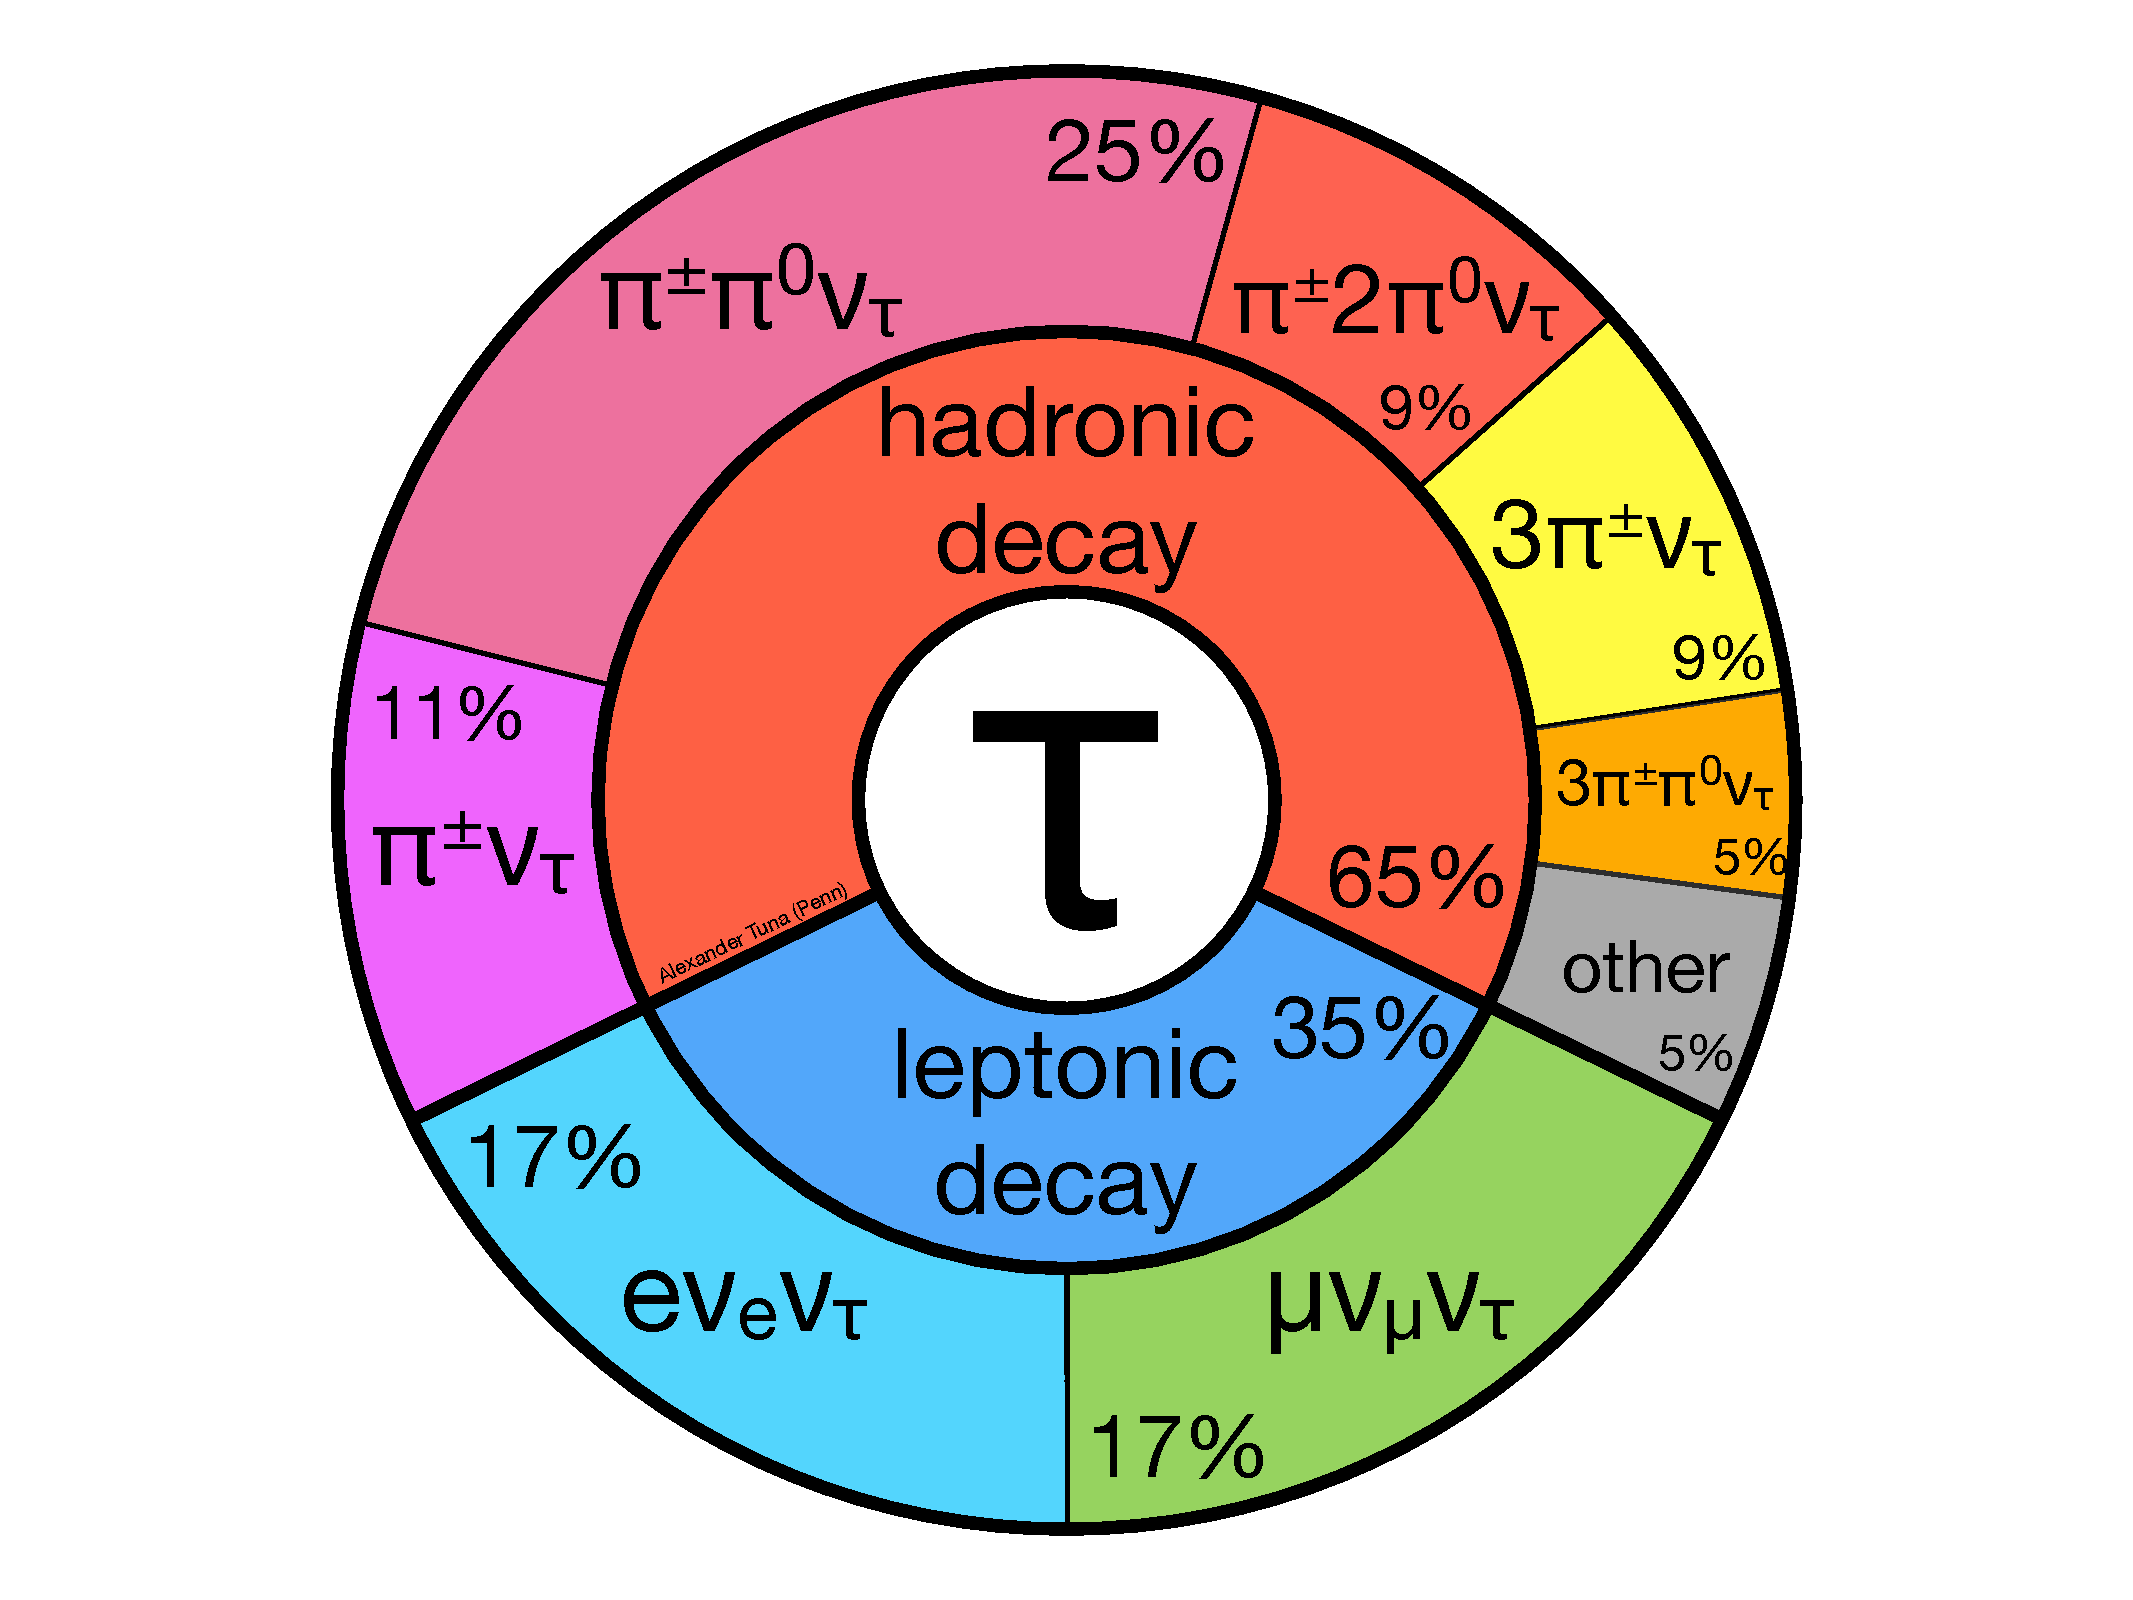
\includegraphics[width=0.48\textwidth]{figures/piecharts/taudecay}
  \caption{Variables.}
  \label{fig:taus-decaypie}
\end{figure}

% ----------------------------------------------------------------------------------

\section{Leptonic tau decays, $\taul$}
\label{sec:taus-leptons}

At ATLAS, light leptons from tau lepton decays ($\tauldecay$) are largely indistinguishable from prompt leptons from $W$ and $Z$ decays. They are typically less energetic due to the presence of two additional neutrinos in the tau lepton decay (e.g., $\Wlv$ versus $\Wtauvlvvv$), but for identification purposes, the only distinguishing features arise from the displaced tau vertex. This displacement is often quantified by the transverse distance of closest approach $d_0$ of the light lepton to the production (``primary'') vertex. But given the short lifetime of tau leptons, the discrimination power is weak. These properties are shown in \cref{fig:taus-leptonpt}.

\begin{figure}[tp]
  \centering
  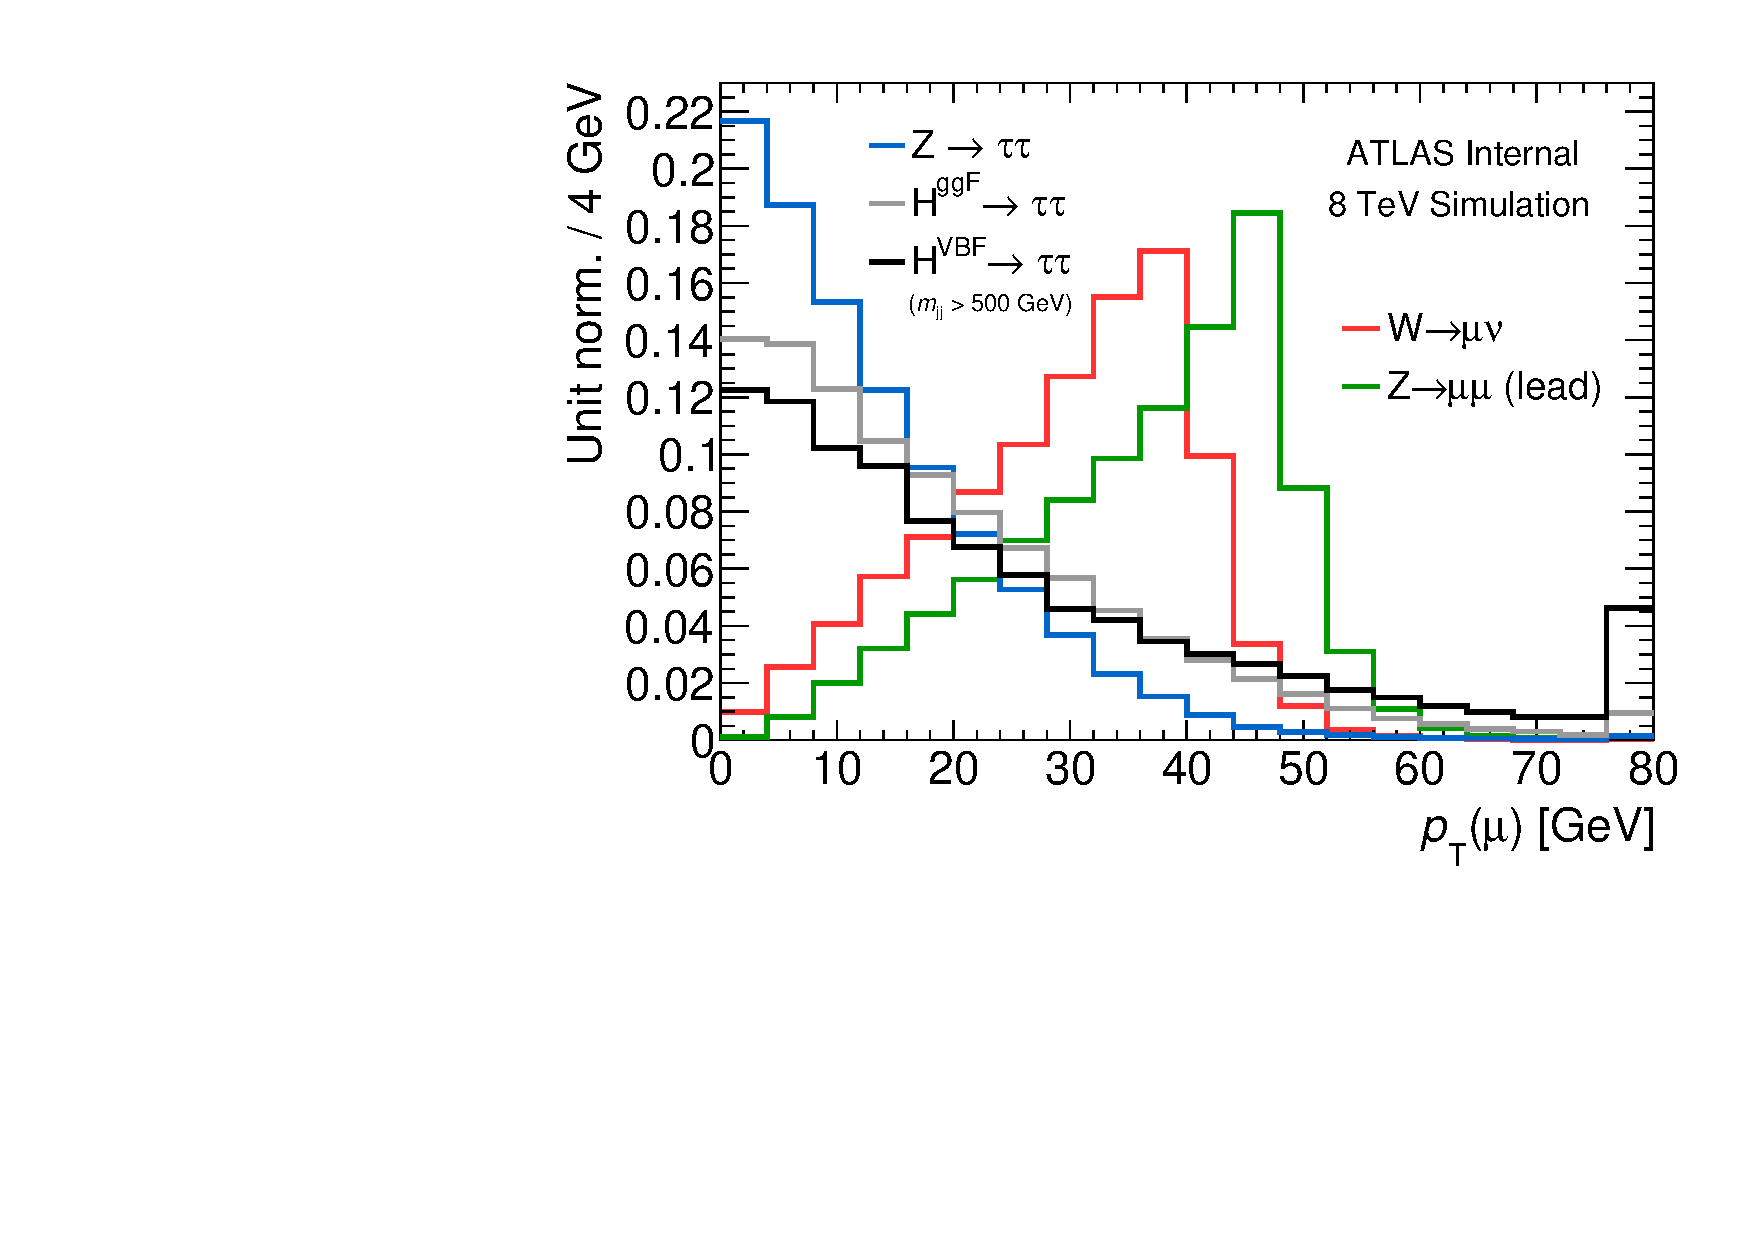
\includegraphics[width=0.48\textwidth]{figures/tauperformance/leptonsfromtausaresoft}
  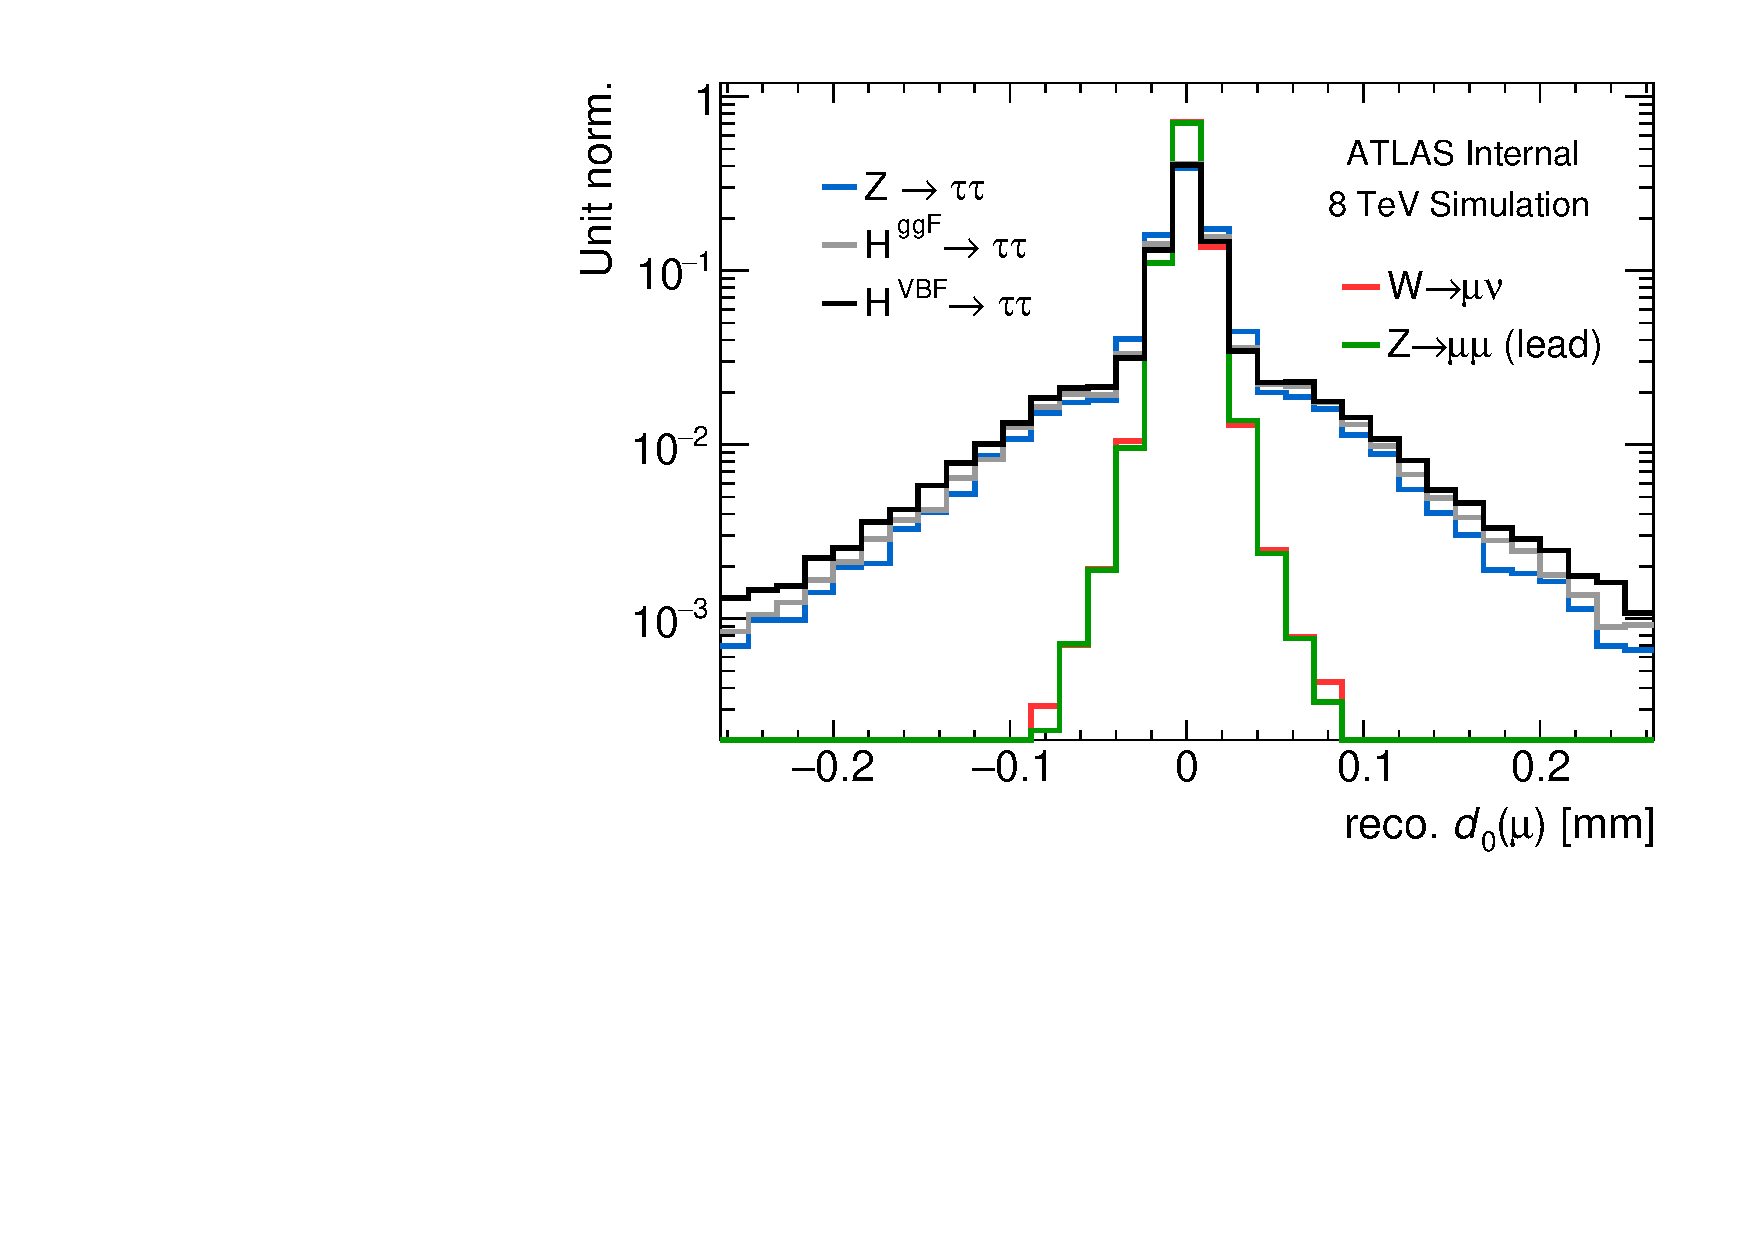
\includegraphics[width=0.48\textwidth]{figures/tauperformance/leptond0}
  \caption{True $\pt$ and reconstructed $d_0$ for muons from simulated $W$, $Z$, and tau lepton decays. Muons from tau lepton decays are shown for $\Ztautau$, $\ggFHtautau$, and $\VBFHtautau$ processes.}
  \label{fig:taus-leptonpt}
\end{figure}

% ----------------------------------------------------------------------------------

\section{Hadronic tau decays, $\tauh$}
\label{sec:taus-hadrons}

This sections follows a recent ATLAS publication describing $\tauh$ performance in Run-I~\cite{PERF-2013-06}.

\subsection{Reconstruction}

\subsubsection{Calorimeter seeding}

$\tauh$ candidates are seeded by the collection of jets formed by the anti-$k_t$ algorithm with distance parameter $R=0.4$, which groups the set of reconstructed three-dimensional calorimeter TopoClusters into jet objects. These TopoClusters are calibrated using a local hadronic calibration (LC). Jets are required to have $\pt > 10 \GeV$ and $|\eta| < 2.5$ to qualify as a seed for a $\tauh$ candidate. The initial $\tauh$ four-momentum is calculated by summing the TopoClusters within $\Delta R < 0.2$ of the barycenter of the jet seed, where the $\tauh$ mass is assume to be zero.

\subsubsection{Track and vertex association}

Tracking and vertexing for $\tauh$ occurs in three steps. First, all tracks are collected within $\Delta R < 0.2$ of the jet seed which pass quality criteria described later, but for which no impact parameter requirements are made. Second, the tau vertex (TV) is defined as the reconstructed vertex which maximizes the fraction of track momenta originating from that vertex versus total track momenta, referred to as the tau vertex fraction:
%
\begin{equation}
  \begin{split}
    \text{TVF}(\text{vertex}) &= \frac{\sum \pt^\text{tracks associated to vertex}}{\sum \pt^\text{tracks}} \\
  \end{split}
  \label{eqn:taus-tvf}
\end{equation}
%
This vertex association is called the Tau Jet Vertex Association algorithm, and it helps ensure robustness against harsh pileup conditions, as shown in \cref{fig:taus-tjva}.

\begin{figure}[tp]
  \centering
  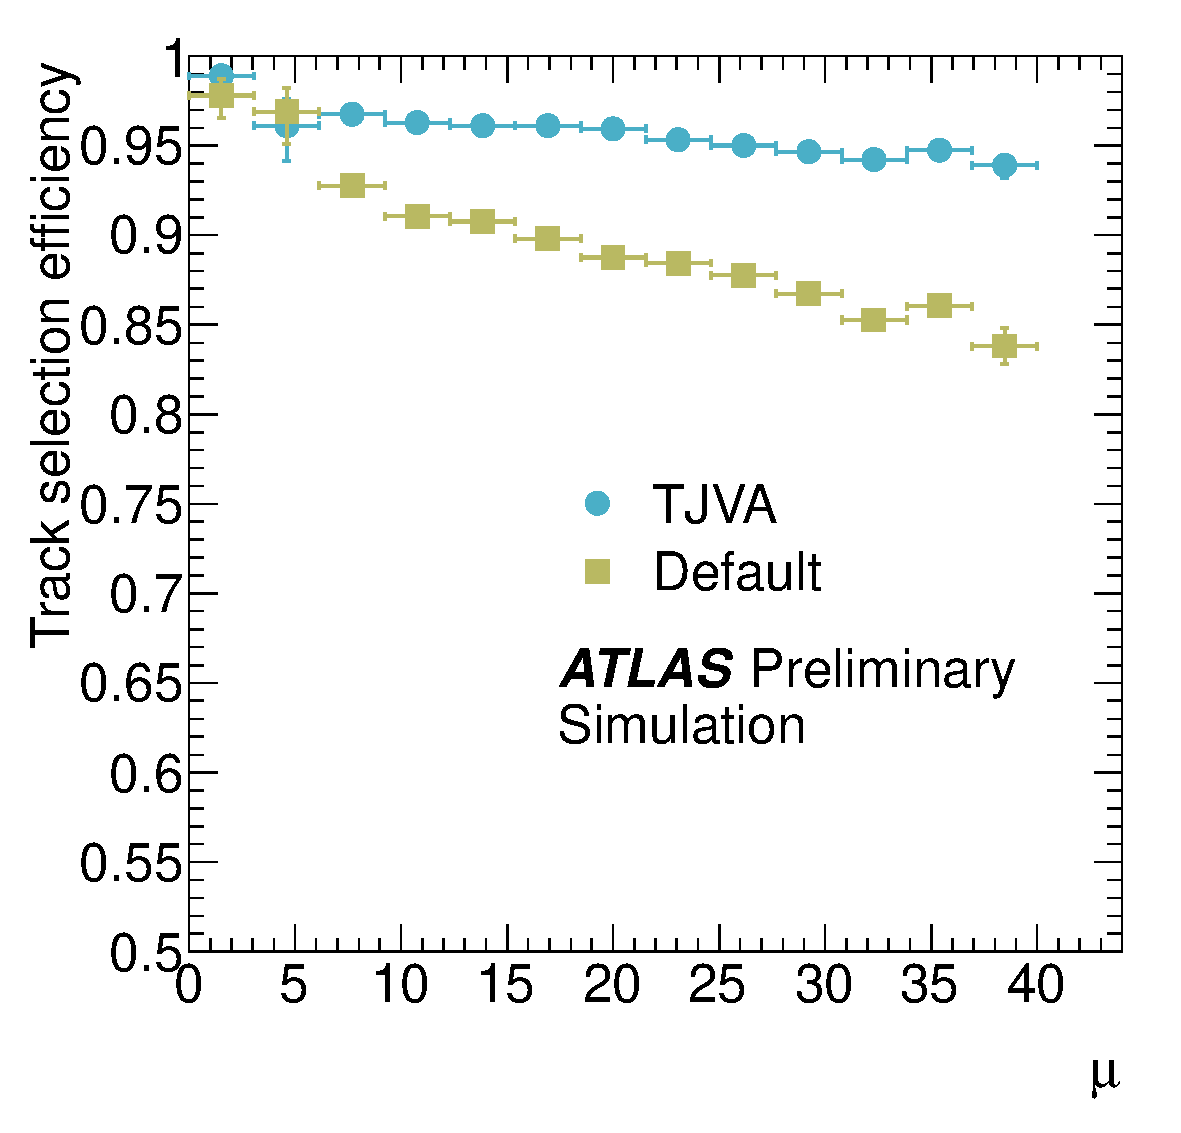
\includegraphics[width=0.48\textwidth]{figures/ATLAS-CONF-2012-142/fig_01a}
  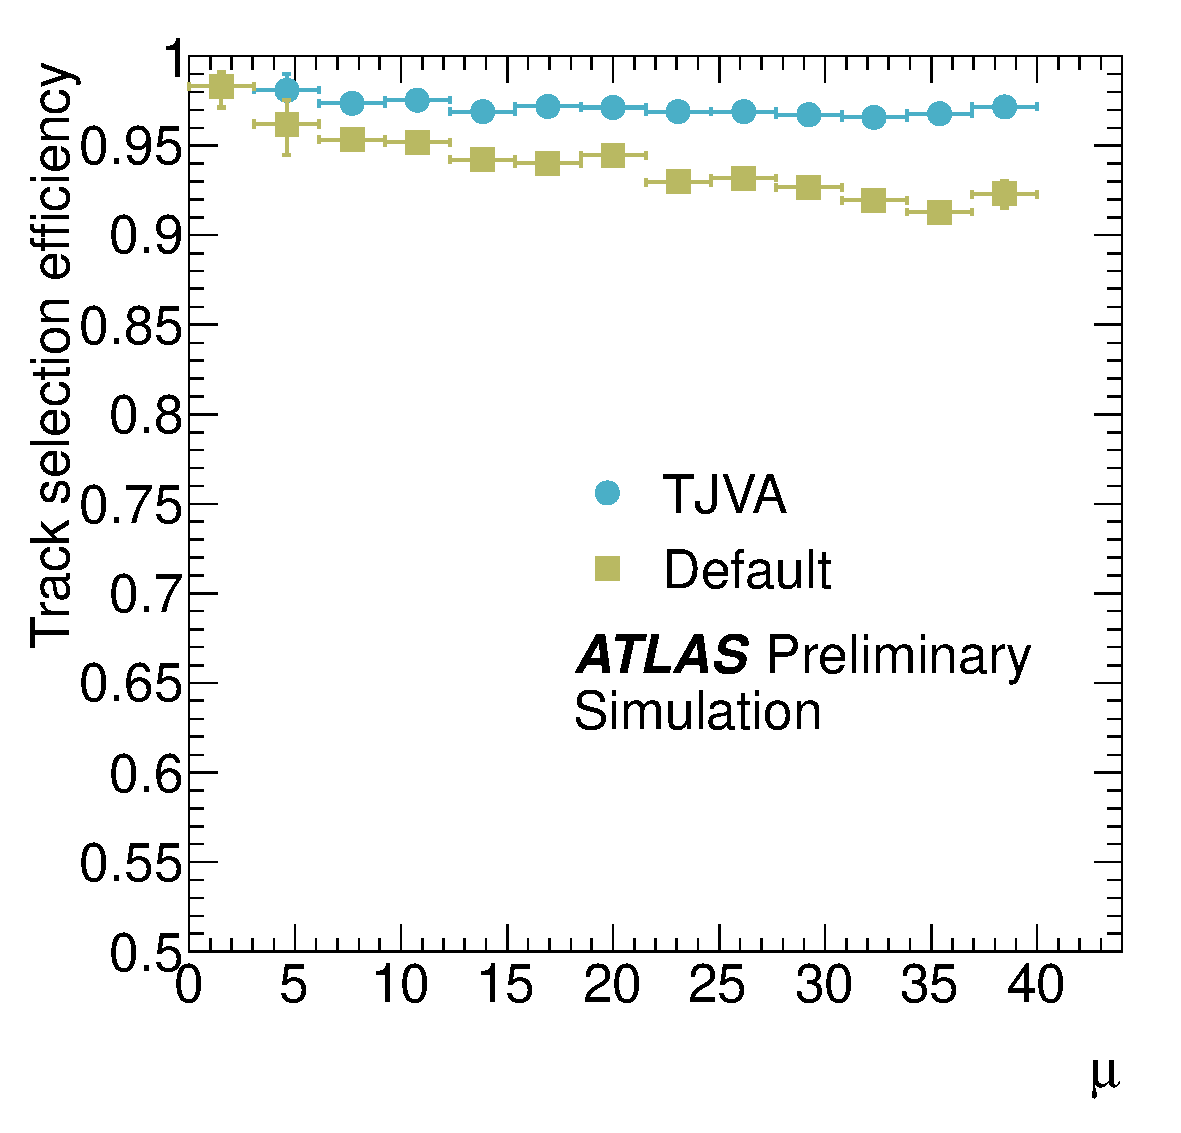
\includegraphics[width=0.48\textwidth]{figures/ATLAS-CONF-2012-142/fig_01b}
  \caption{Variables.}
  \label{fig:taus-tjva}
\end{figure}

Last, the set of tracks is reduced by making additional impact parameters requirements with respect to the TV. The full set of track selection criteria are:
%
\begin{itemize}
    \item $\pt > 1~\mathrm{GeV}$,
    \item at least two hits in the pixel subdetector,
    \item at least seven hits in the pixel and SCT subdetectors combined,
    \item $|d_{0,\text{TV}}| < 1.0~\mathrm{mm}$,
    \item $|z_{0,\text{TV}} \, \sin{\theta}| < 1.5~\mathrm{mm}$
\end{itemize}
%
This set of tracks is used when classifying the $\tauh$ candidate track multiplicity. For identification purposes, tracks in the \textit{isolation region} $0.2 < \Delta R < 0.4$ are also required to pass these criteria.

\subsubsection{Calibration}

A correction to the $\tauh$ energy is applied to account for biases, such as effects from pileup, the underlying event, and clusters falling out of the $\Delta R = 0.2$ cone. This correction is derived in simulated $\Ztautau$, $\Wtaunu$, and $\Zptautau$ events where the true visible $\tauh$ energy $\Etruevis$ is known. It is derived as a function of the pre-calibrated $\tauh$ energy $\ErecoLC$ and $\eta$ and shown in \cref{fig:taus-calibration}. Small additional corrections are applied to account for biases from pileup and poorly instrumented regions of the detector. The resulting $\tauh$ energy resolution is shown in \cref{fig:taus-resolution}.

\begin{figure}[tp]
  \centering
  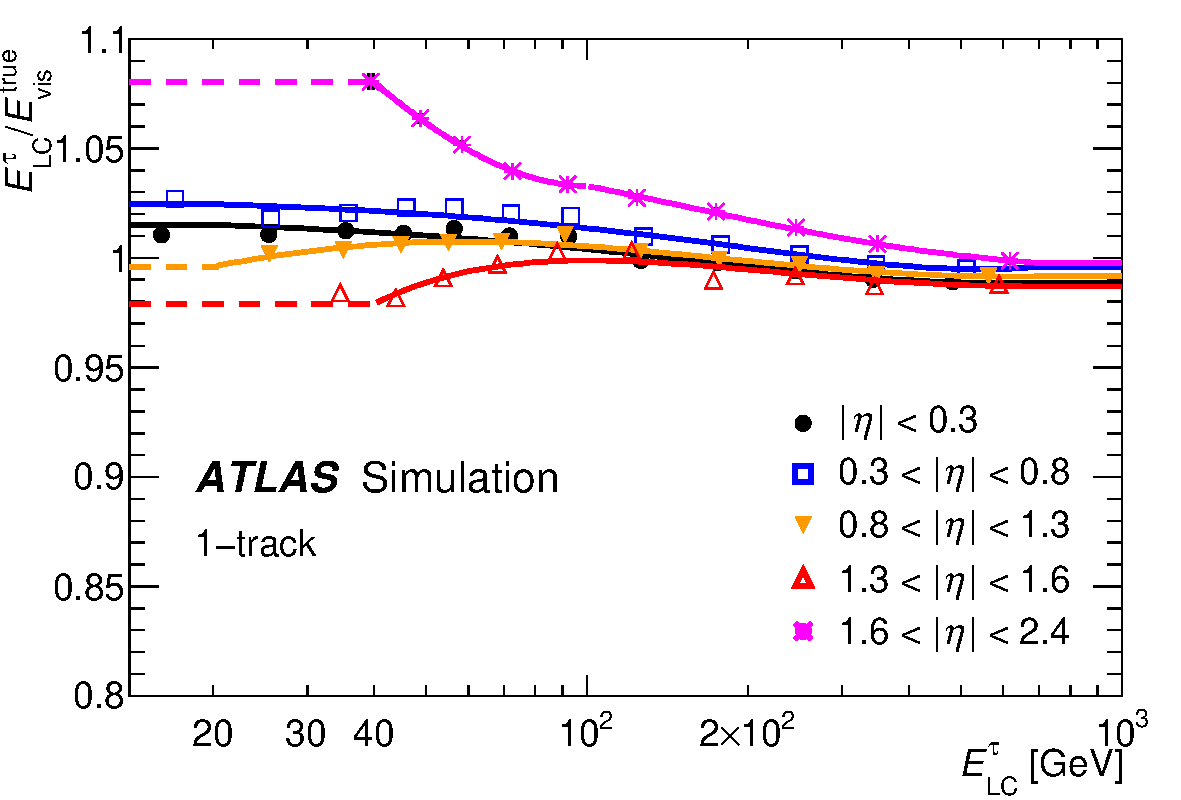
\includegraphics[width=0.48\textwidth]{figures/PERF-2013-06/fig_15a}
  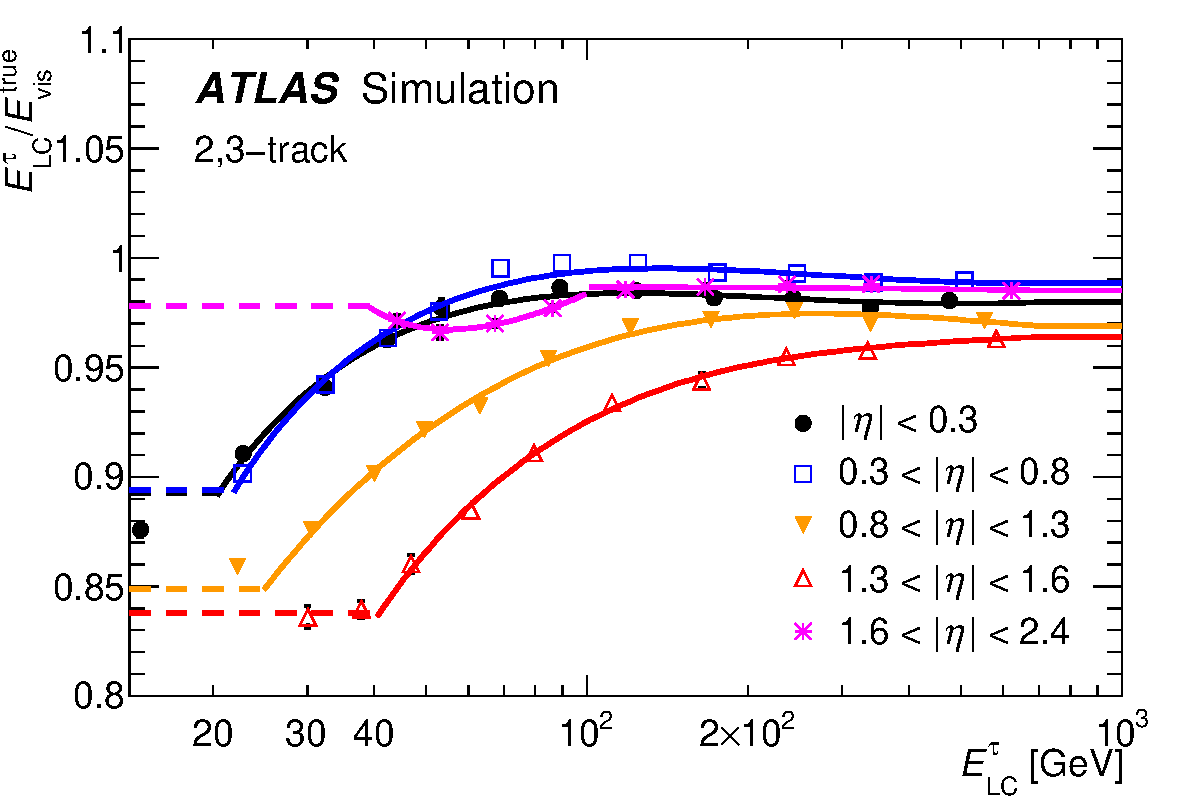
\includegraphics[width=0.48\textwidth]{figures/PERF-2013-06/fig_15b}
  \caption{Variables.}
  \label{fig:taus-calibration}
\end{figure}

\begin{figure}[tp]
  \centering
  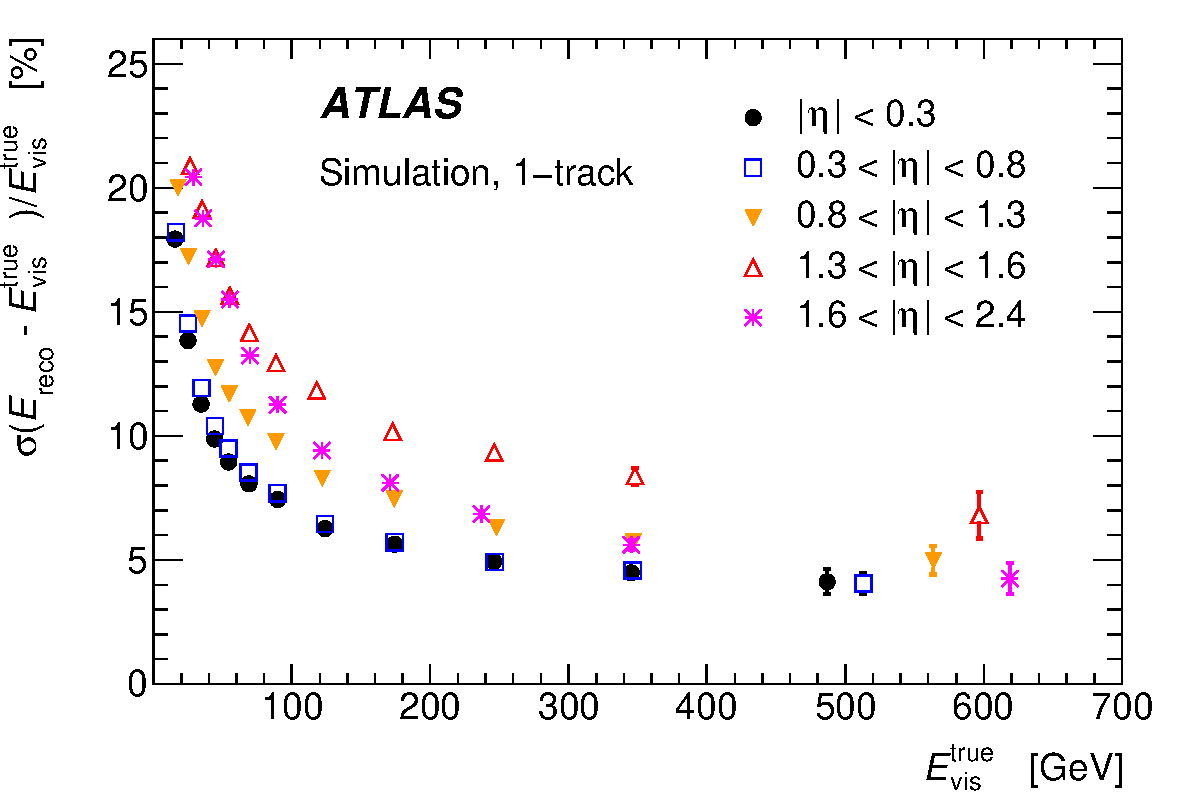
\includegraphics[width=0.48\textwidth]{figures/PERF-2013-06/fig_16a}
  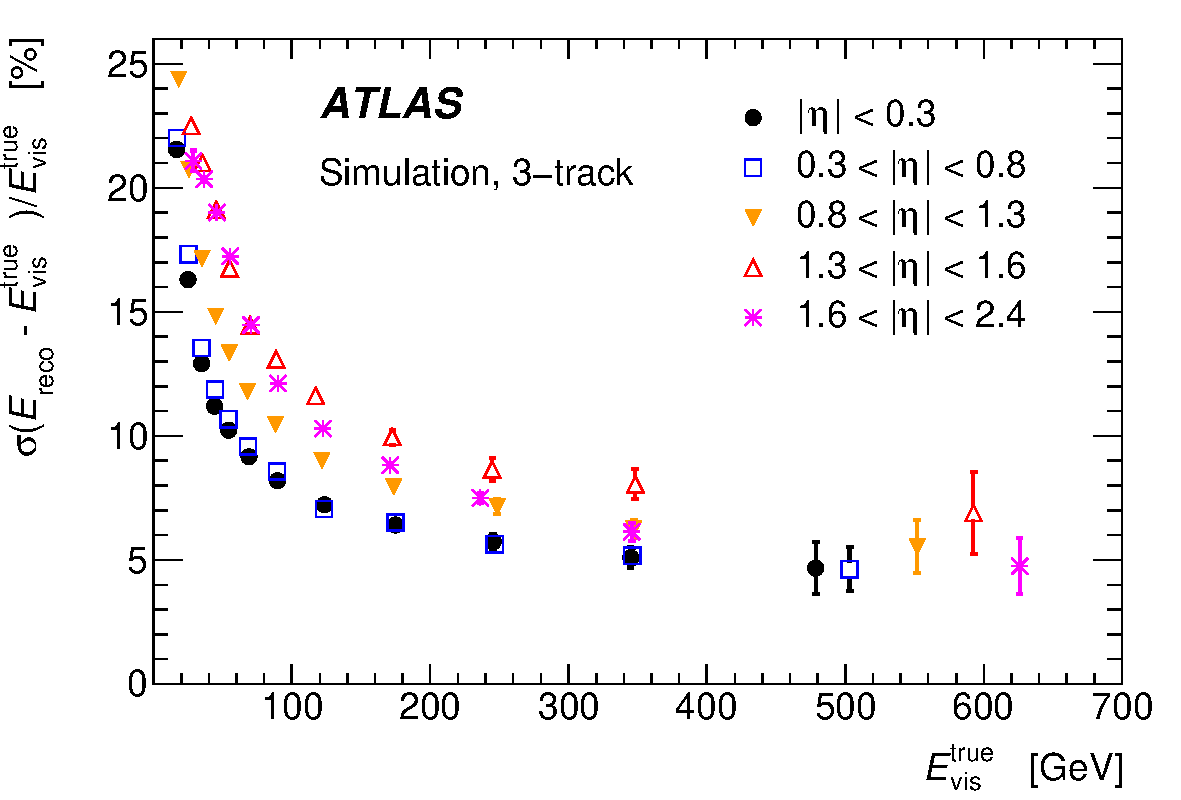
\includegraphics[width=0.48\textwidth]{figures/PERF-2013-06/fig_16b}
  \caption{Variables.}
  \label{fig:taus-resolution}
\end{figure}

Data-driven corrections for and uncertainties on the $\tauh$ energy calibration are derived in two ways: the \textit{deconvolution method} and the \textit{in-situ} method. The deconvolution method relies on the $\tauh$ having a known composition of charged and neutral hadrons such that the response can be decomposed into individual sources. For charged hadrons, the response is estimated from test beam measurements and simulation with varied hadronic shower models. For electromagnetic showers from neutral pion decays, the response is estimated from $\Zee$.

The in-situ method relies on the sensitivity of the visible $\mtautau$ in $\Ztaultauh$ events to the $\tauh$ energy. Relative to $\tauh$, the lepton energy is precisely calibrated and validated in data with $\Zll$ events. These events are selected in data by requiring exactly one isolated muon, exactly one identified $\tauh$, and some additional kinematic cuts to suppress non-$\Ztaultauh$ events. The $\tauh$ energy is then allowed to float like $(1 + \alpha)E_\text{T}$, and the effect is propagated to the visible $\mtautau$ spectrum. The data is then adjusted by the parameter $\alpha$ to match the simulated prediction, which has already been corrected to $\Etruevis$. The measured $\alpha$, called the \textit{TES shift}, is:
%
\begin{equation}
  \begin{split}
    \alpha_\text{1-track} &= 0.8\% \pm 1.3\% \text{ (stat.) } \pm 0.6\% \text{ (syst.) } \\
    \alpha_\text{3-track} &= 1.1\% \pm 1.4\% \text{ (stat.) } \pm 0.7\% \text{ (syst.) } \\
  \end{split}
  \label{eqn:taus-tesshift}
\end{equation}
%

\section{Identification}

As a high energy hadron collider, the overwhelming majority of particles observed by ATLAS are hadrons. Distinguishing these QCD jets from $\tauh$ is then of huge consequence. The properties with discriminating power can be broadly grouped into three categories:
%
\begin{itemize}
    \item \textbf{Track multiplicity}. $\tauh$ tend to have 1 or 3 associated tracks, where no such specificity is expected for jets.
    \item \textbf{Narrowness}. $\tauh$ tend to be more narrow in the tracker and calorimeter since tau leptons from electroweak decays are boosted.
    \item \textbf{Displaced vertex}. Tracks from $\tauh$ tend to be more displaced from the primary vertex than tracks in jets due to the finite tau lepton lifetime.
\end{itemize}
%


\begin{figure}[tp]
  \centering
  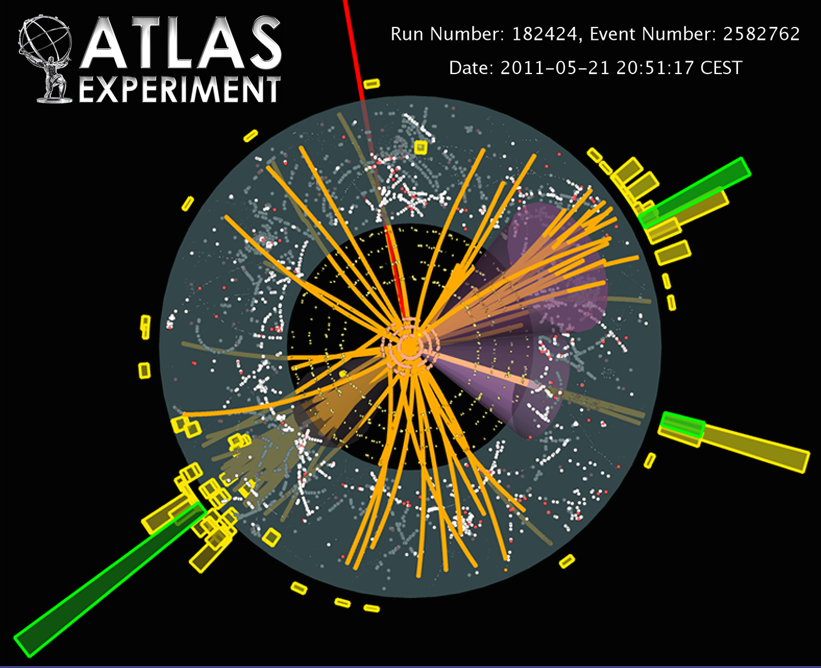
\includegraphics[width=0.95\textwidth]{figures/tauperformance/vp1_3dcocktail_run182424_evt2582762_tttaumu}
  \caption{Variables.}
  \label{fig:taus-eventdisplay}
\end{figure}

\begin{figure}[tp]
  \centering
  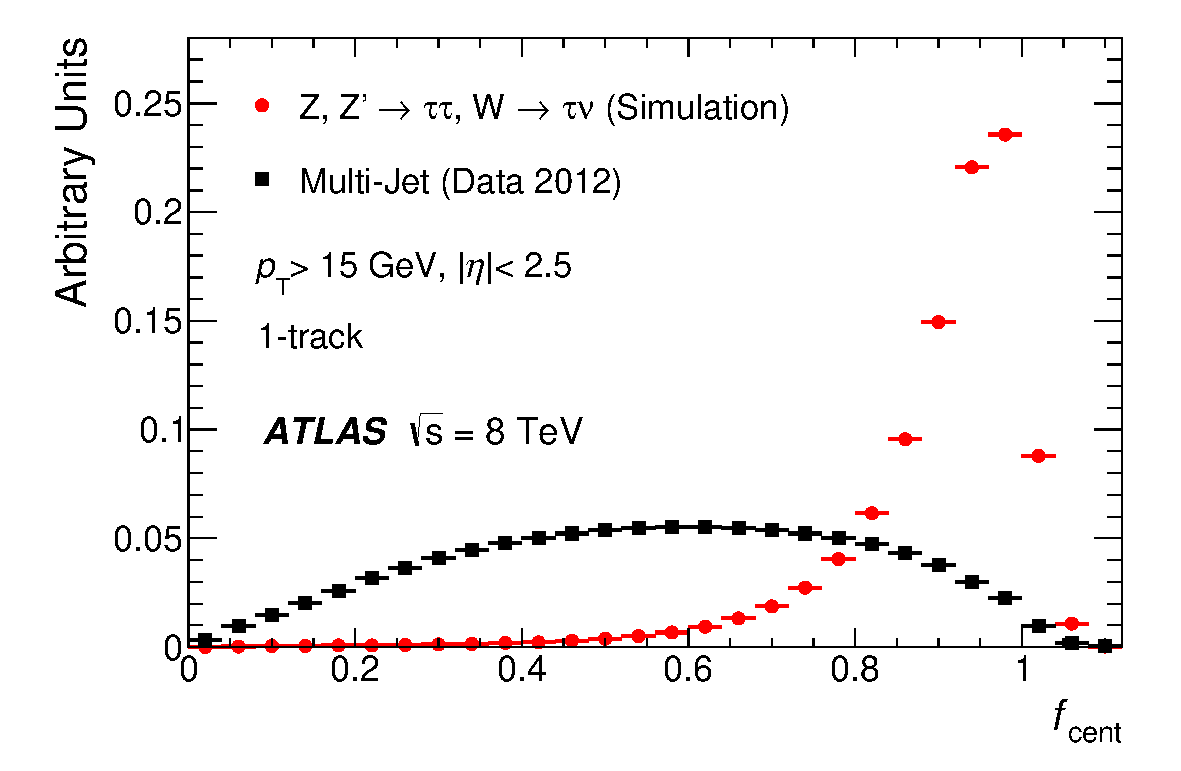
\includegraphics[width=0.48\textwidth]{figures/PERF-2013-06/fig_02a}
  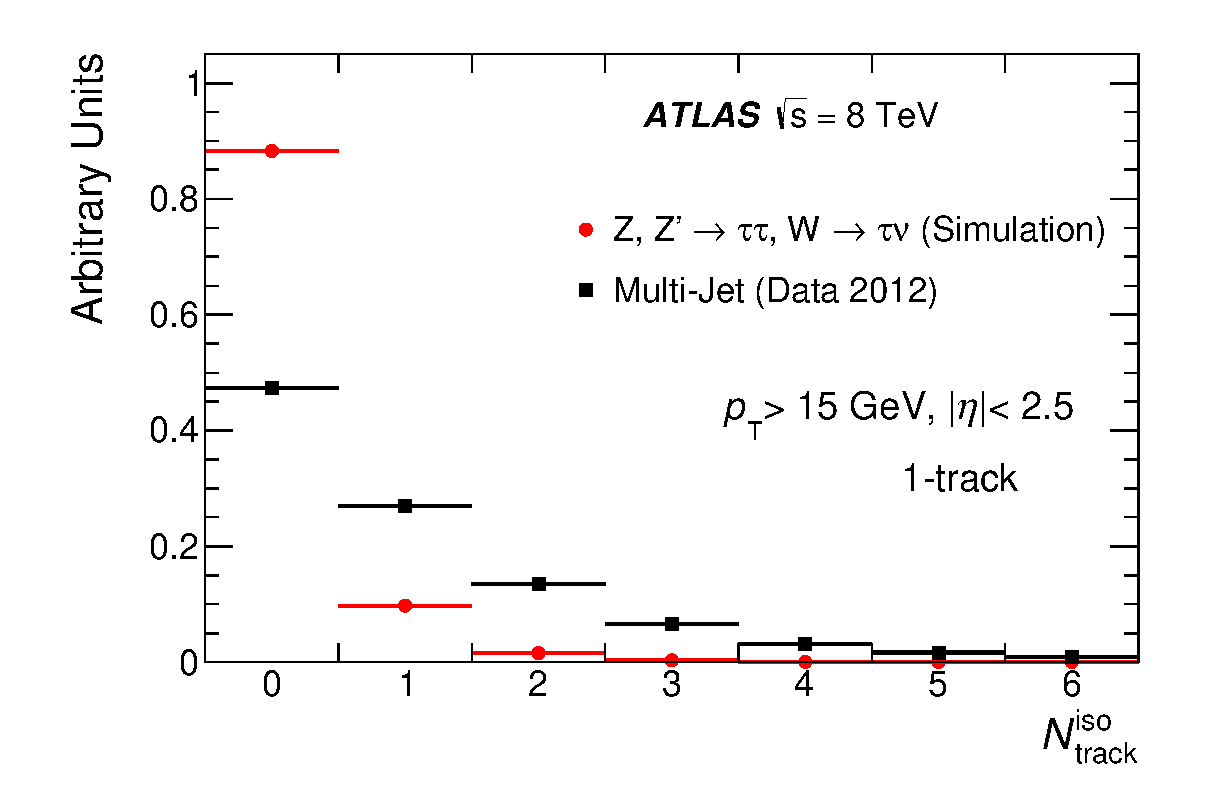
\includegraphics[width=0.48\textwidth]{figures/PERF-2013-06/fig_02b}
  \caption{Variables.}
  \label{fig:taus-id1p}
\end{figure}

\begin{figure}[tp]
  \centering
  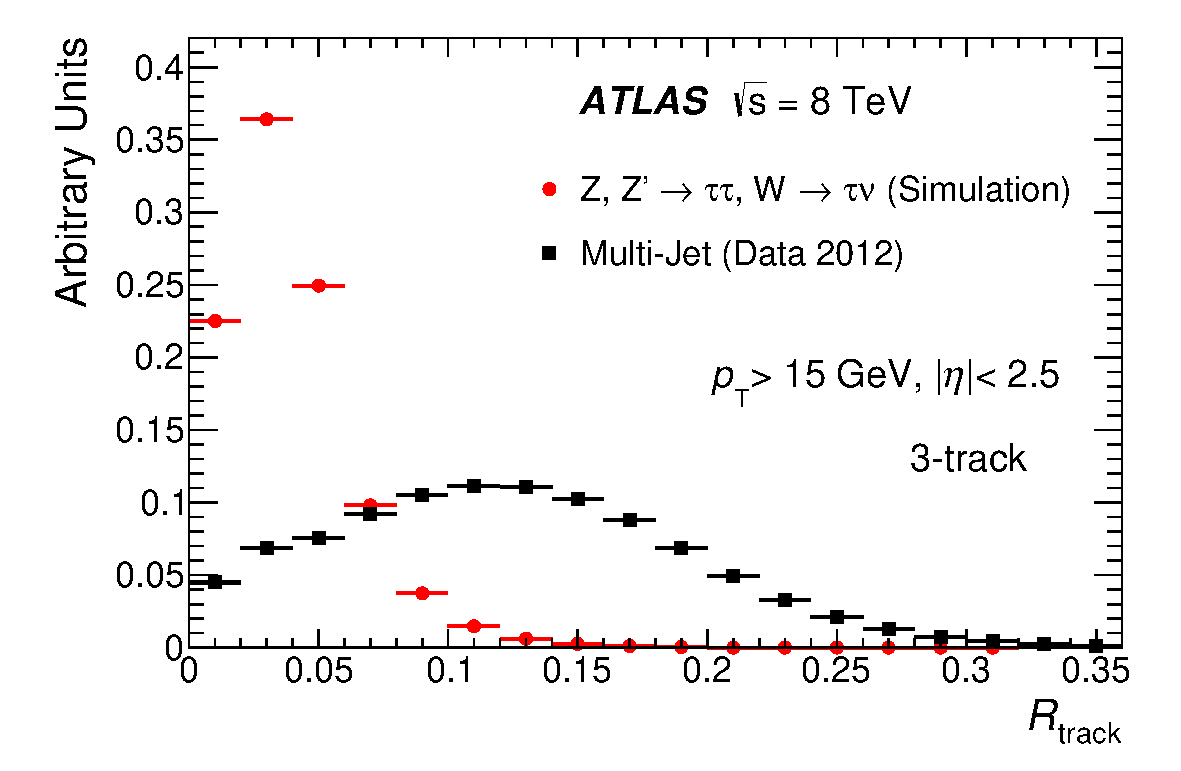
\includegraphics[width=0.48\textwidth]{figures/PERF-2013-06/fig_03a}
  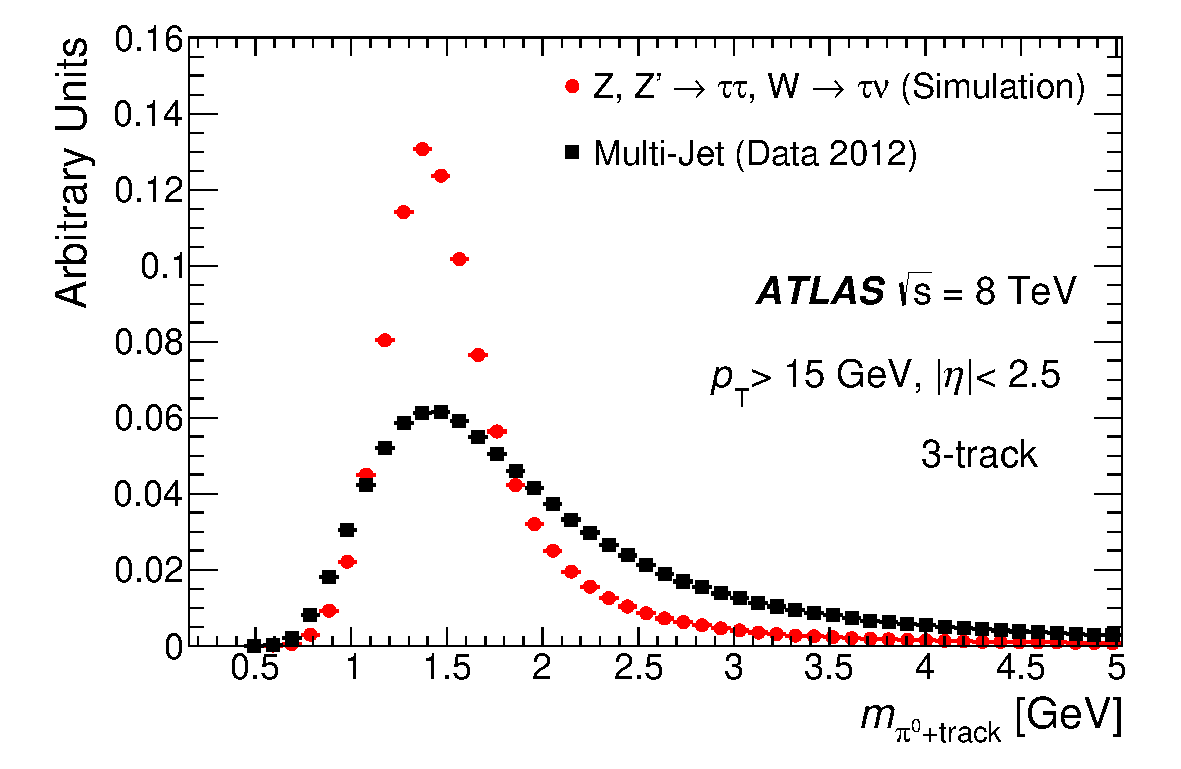
\includegraphics[width=0.48\textwidth]{figures/PERF-2013-06/fig_03b}
  \caption{Variables.}
  \label{fig:taus-id3p}
\end{figure}

\begin{figure}[tp]
  \centering
  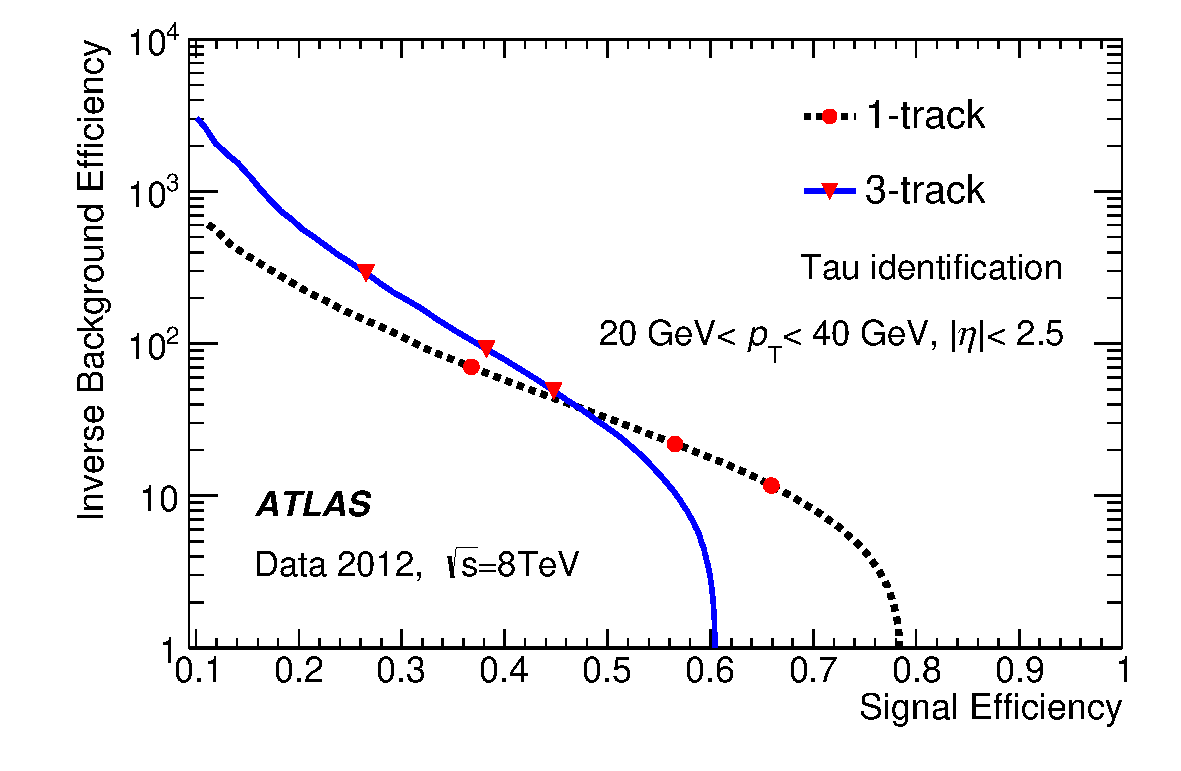
\includegraphics[width=0.48\textwidth]{figures/PERF-2013-06/fig_05a}
  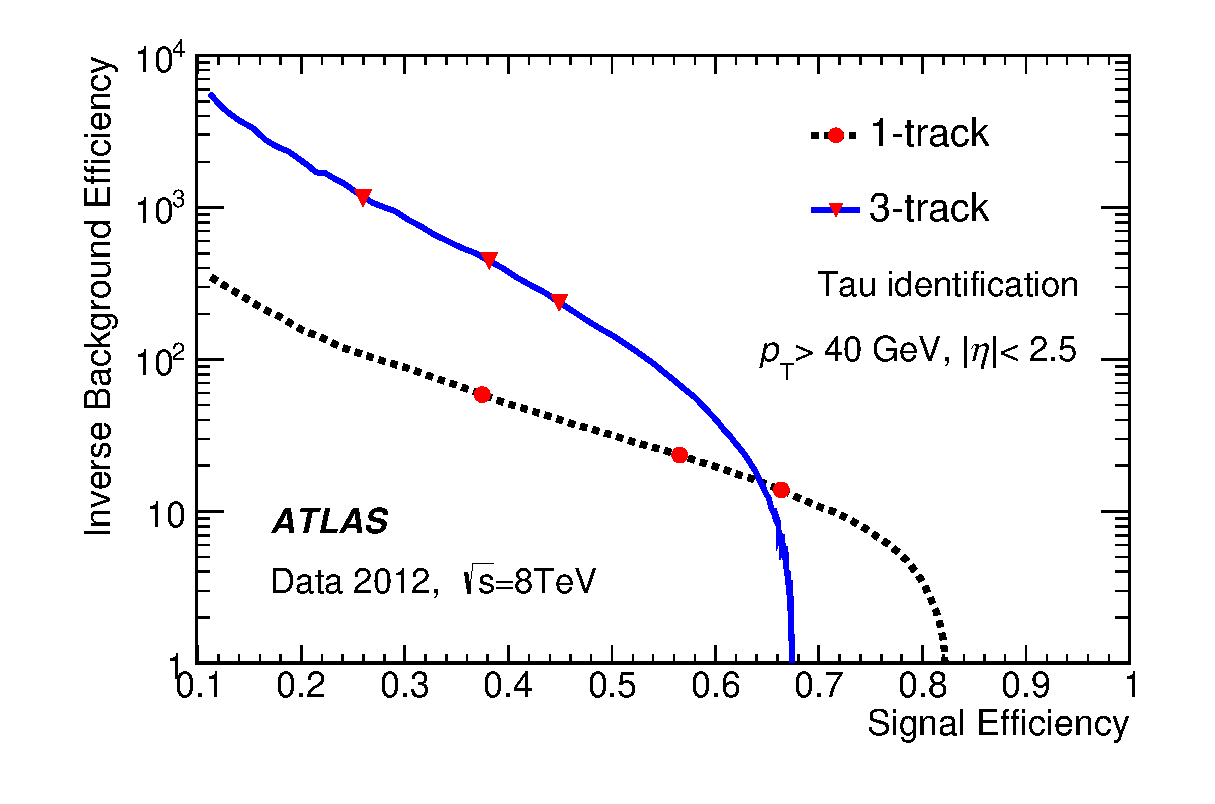
\includegraphics[width=0.48\textwidth]{figures/PERF-2013-06/fig_05b}
  \caption{Variables.}
  \label{fig:taus-idroc}
\end{figure}

\section{Leptons mis-identified as $\tauh$}
\label{sec:taus-leptonfakes}

\subsection{Electrons}

\begin{figure}[tp]
  \centering
  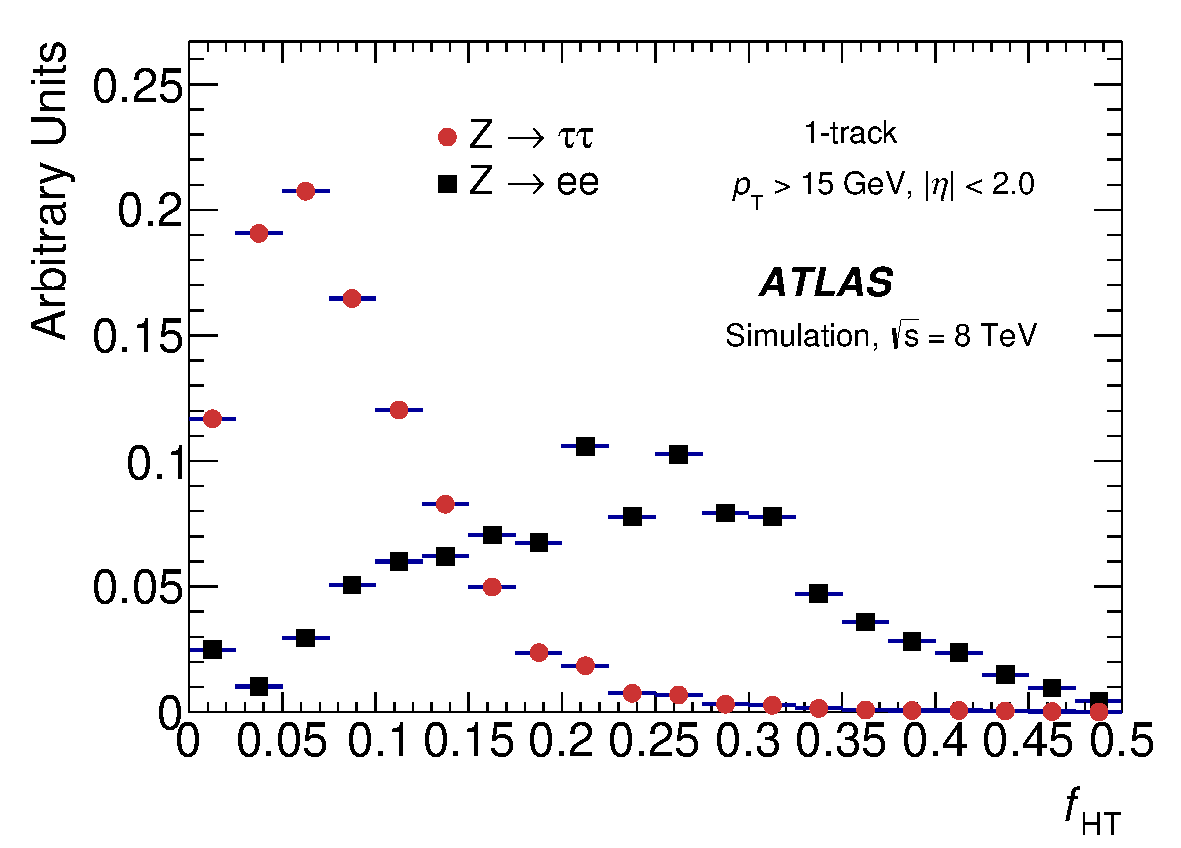
\includegraphics[width=0.48\textwidth]{figures/PERF-2013-06/fig_08a}
  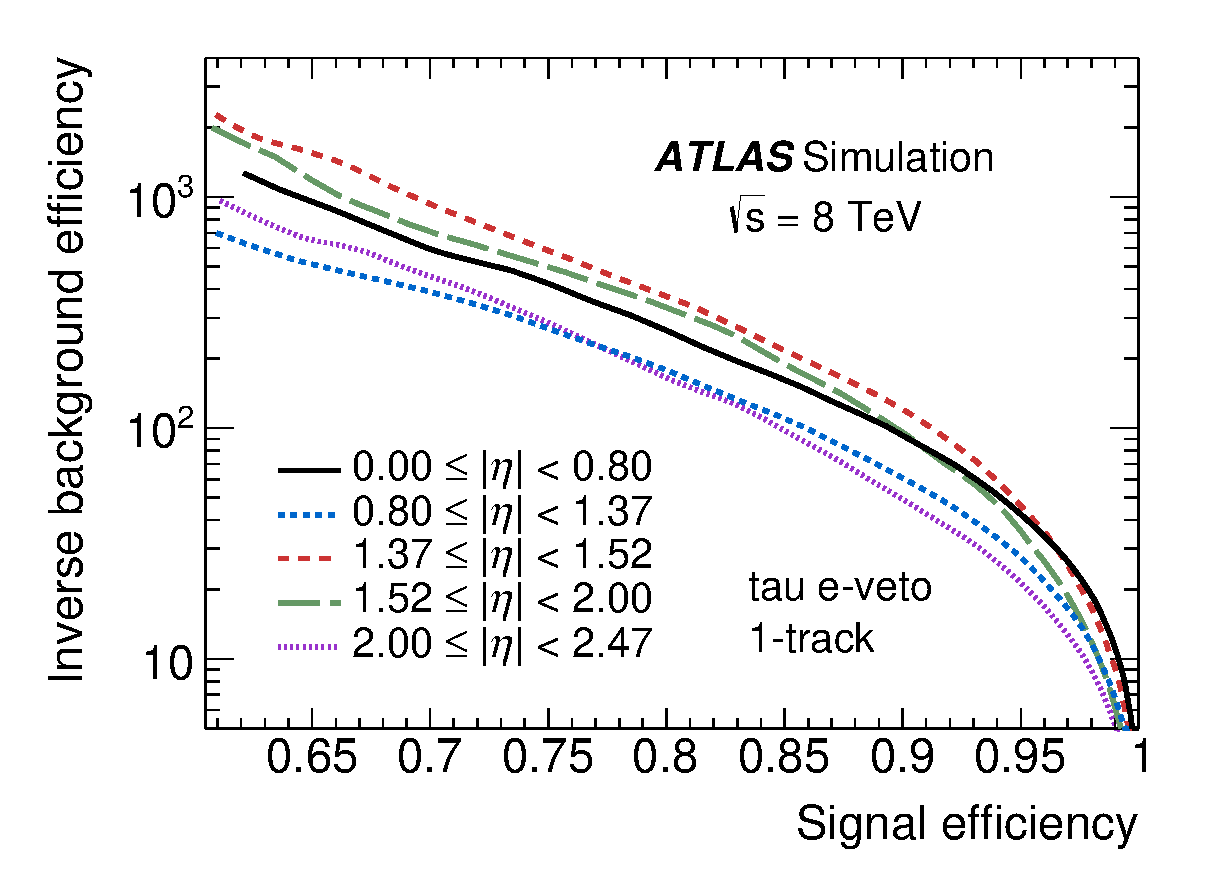
\includegraphics[width=0.48\textwidth]{figures/PERF-2013-06/fig_09}
  \caption{Variables.}
  \label{fig:taus-electronfakes1}
\end{figure}

\begin{figure}[tp]
  \centering
  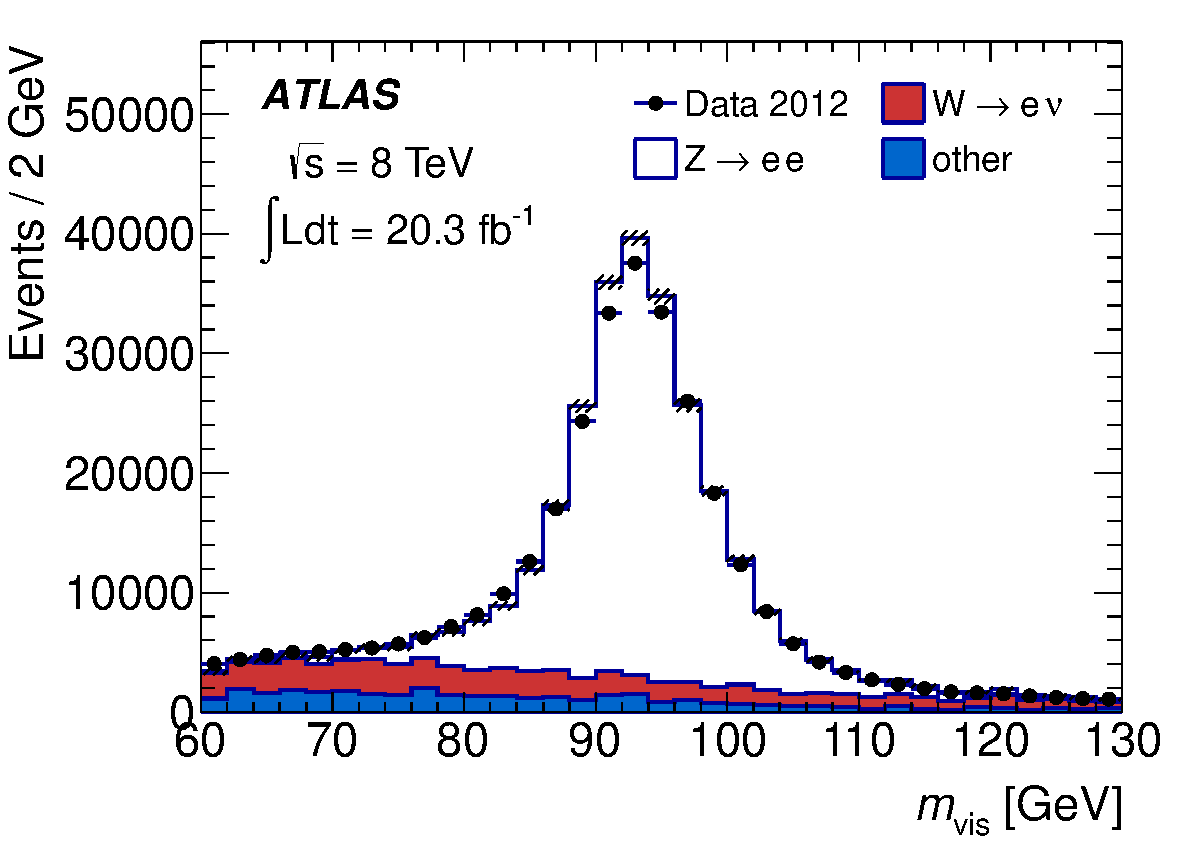
\includegraphics[width=0.48\textwidth]{figures/PERF-2013-06/fig_14a}
  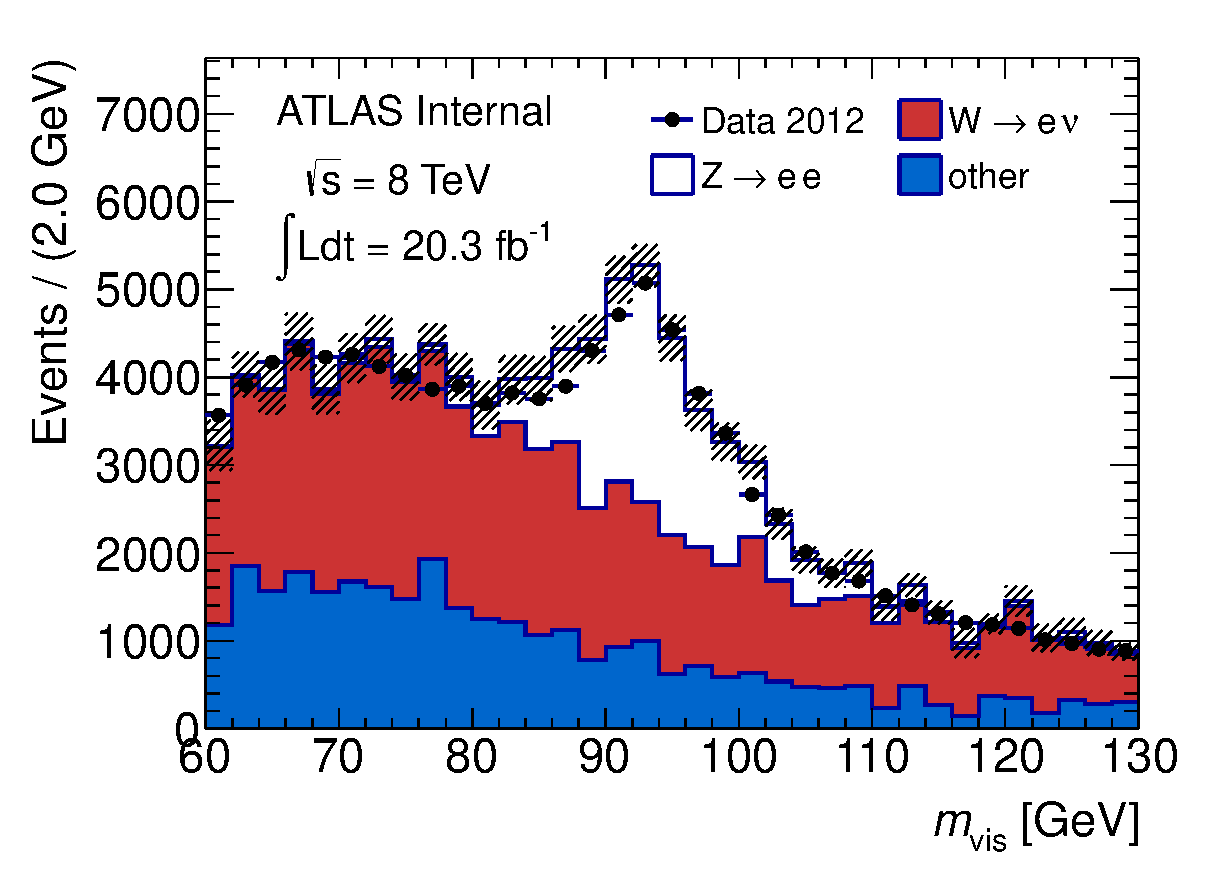
\includegraphics[width=0.48\textwidth]{figures/PERF-2013-06/eveto_mvis_mediumID_loosePPOLR_looseeveto}
  \caption{Variables.}
  \label{fig:taus-electronfakes2}
\end{figure}

\subsection{Muons}

\begin{figure}[tp]
  \centering
  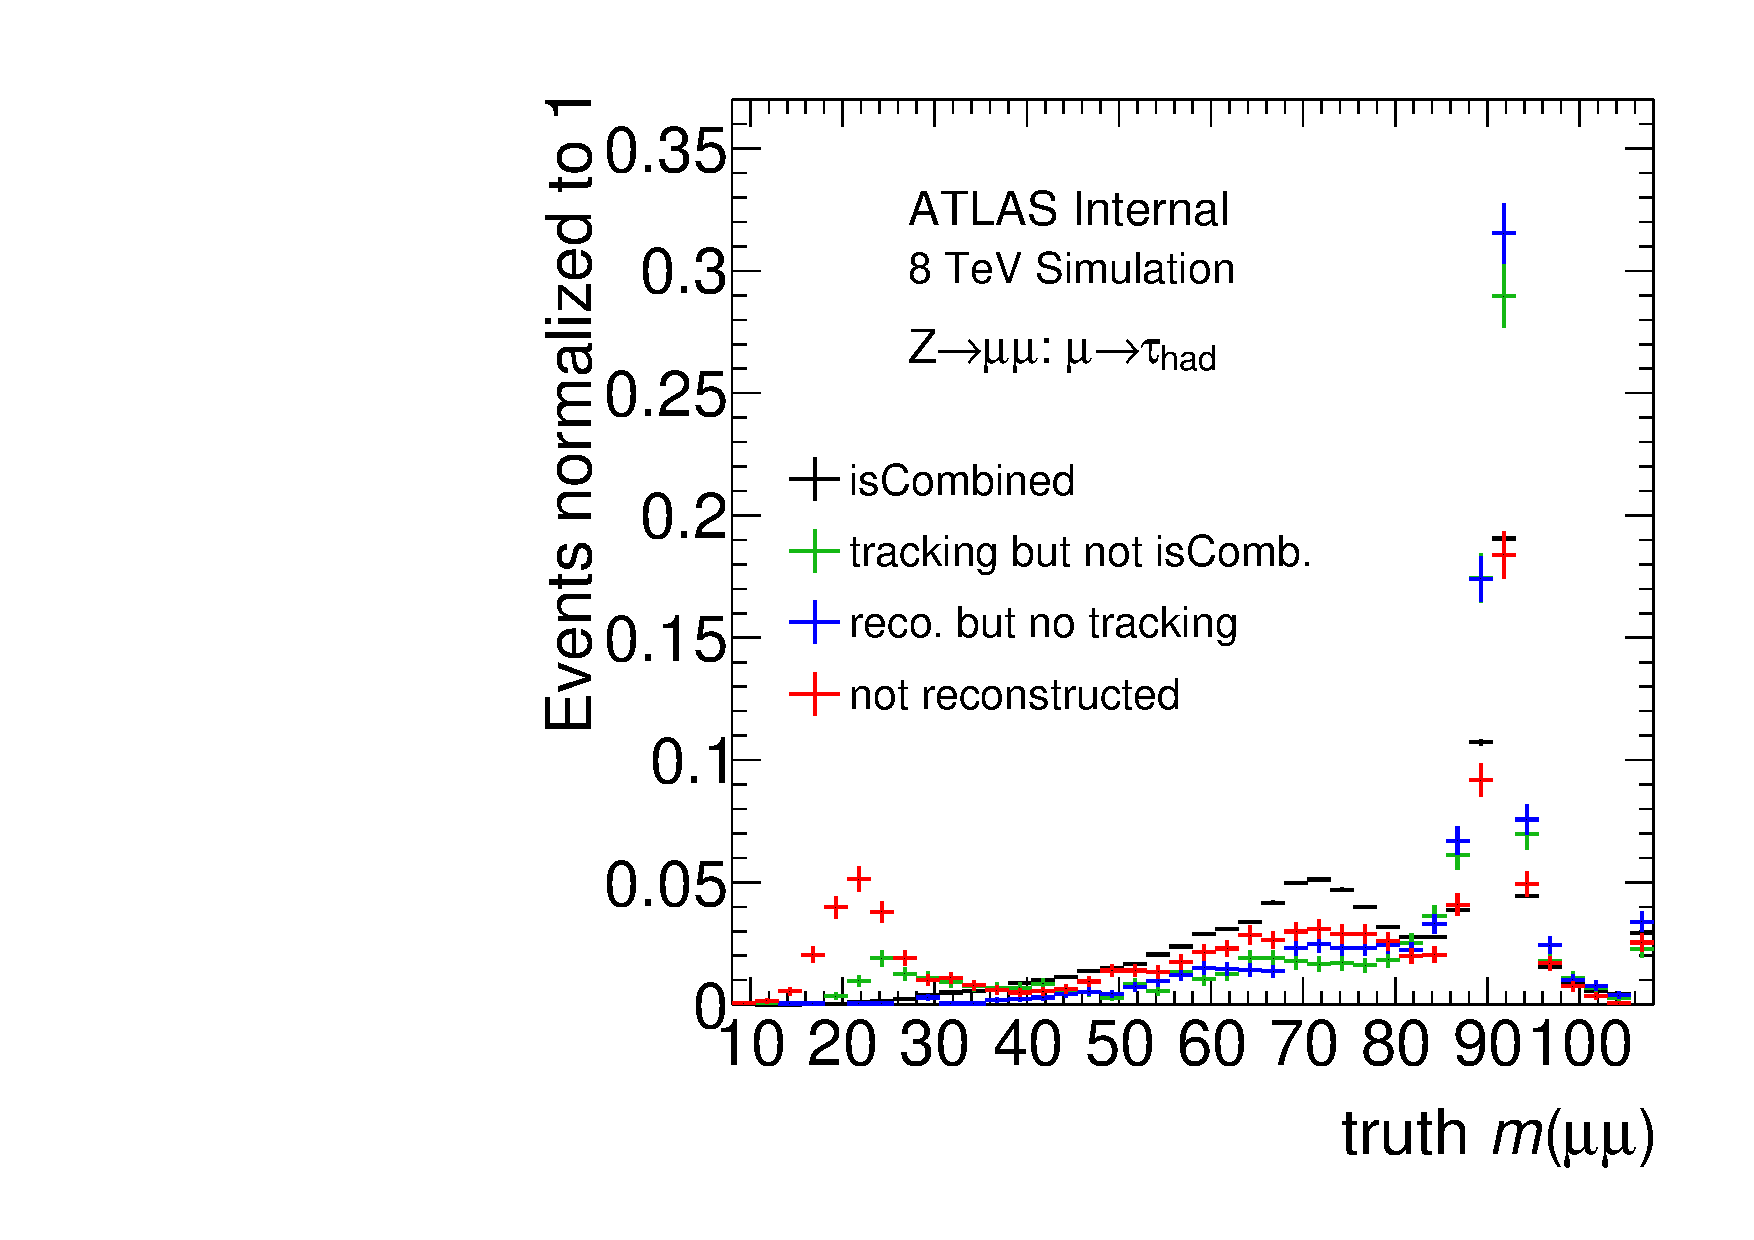
\includegraphics[width=0.48\textwidth]{figures/tauperformance/muonfakes_mll}
  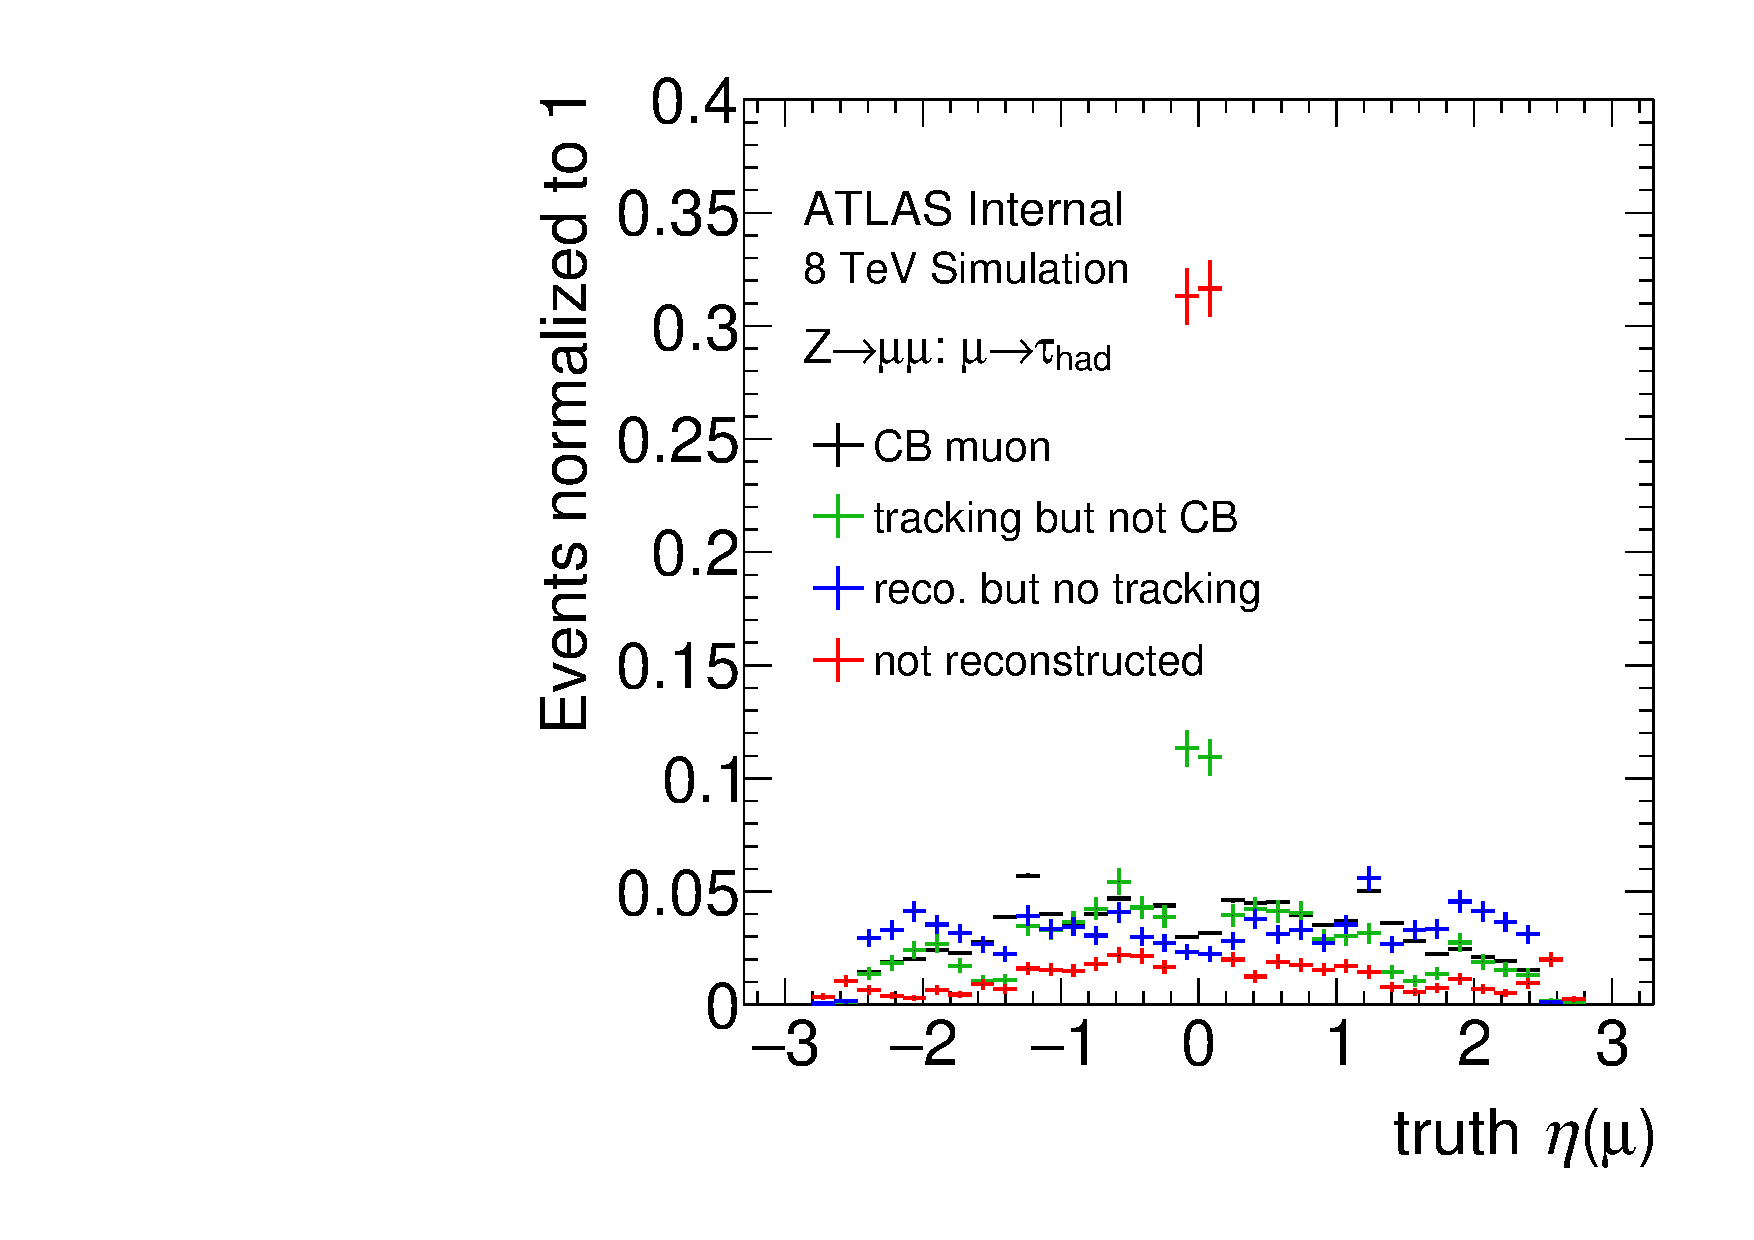
\includegraphics[width=0.48\textwidth]{figures/tauperformance/muonfakes_eta}
  \caption{Variables.}
  \label{fig:taus-muonfakes1}
\end{figure}

\begin{figure}[tp]
  \centering
  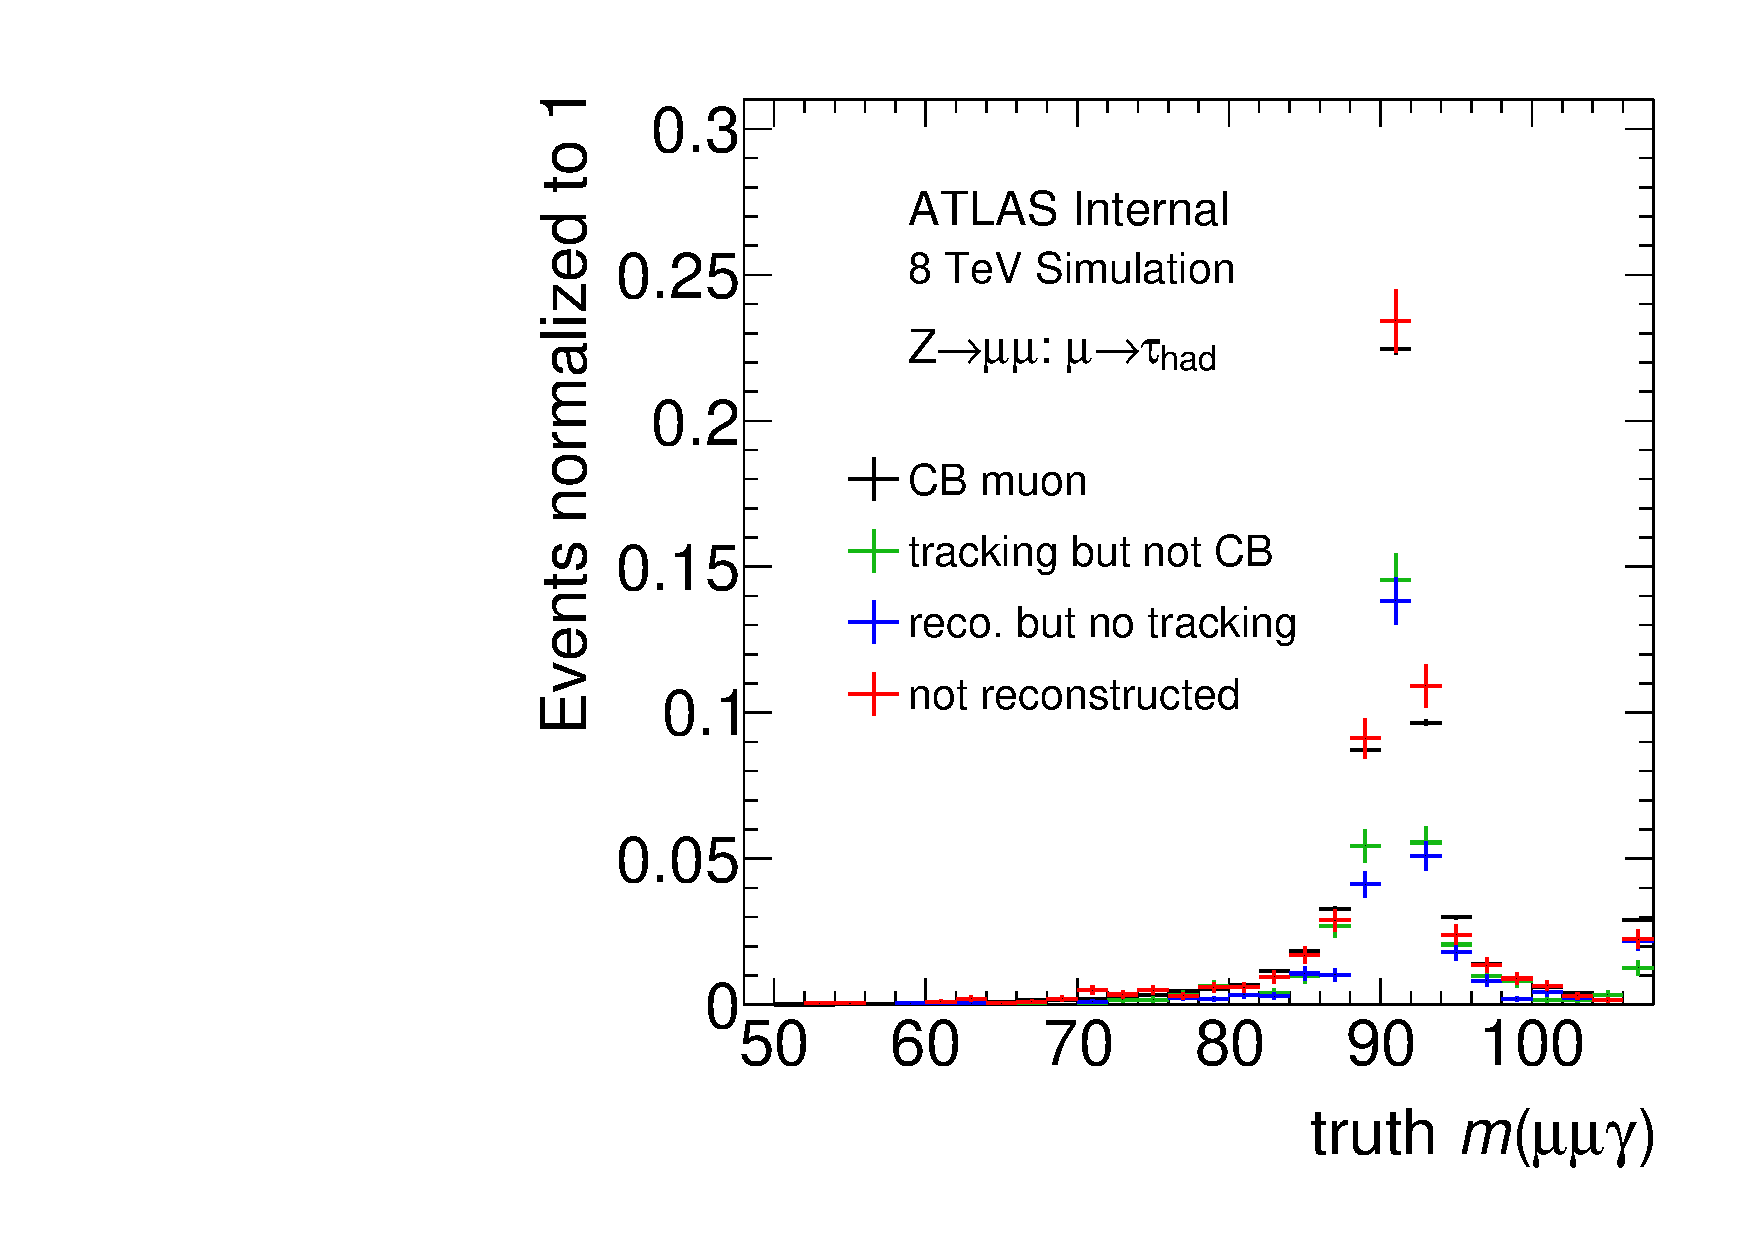
\includegraphics[width=0.48\textwidth]{figures/tauperformance/muonfakes_mlly}
  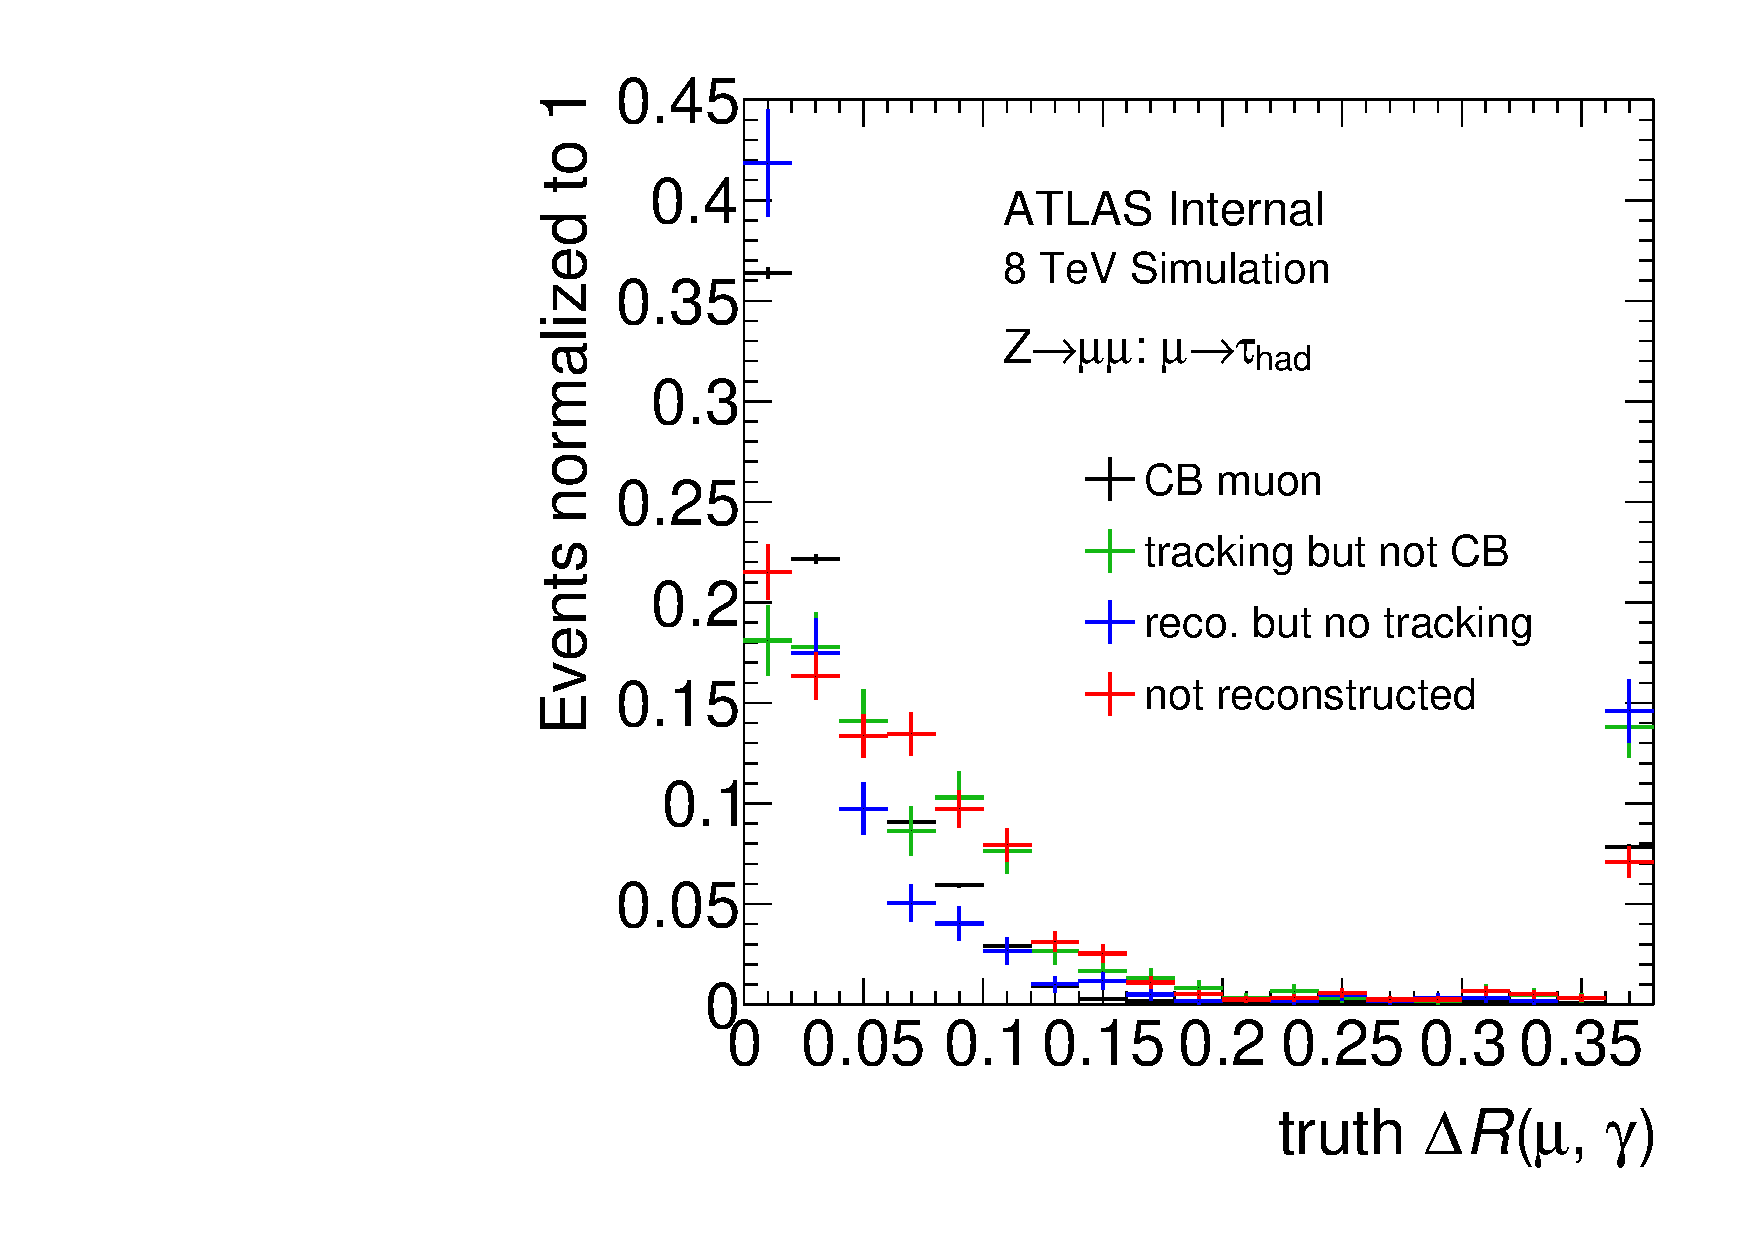
\includegraphics[width=0.48\textwidth]{figures/tauperformance/muonfakes_dR}
  \caption{Variables.}
  \label{fig:taus-muonfakes2}
\end{figure}


